\documentclass[11pt,oneside,openany,report]{jsbook}
%
\usepackage{amsmath,amssymb}
\usepackage{bm}
\usepackage[dvipdfmx]{graphicx}
\usepackage[dvipdfmx]{color}
\usepackage{ascmac}
\usepackage{mathtools}
\usepackage{comment}
\usepackage{subfigure}
\usepackage{algorithm}
\usepackage{algorithmic}
\usepackage{setspace}
\usepackage{multirow}
\usepackage{lscape}
\usepackage{fullpage}

%
%\setlength{\textwidth}{\fullwidth}
%\setlength{\textheight}{50\baselineskip}
\addtolength{\textheight}{\topskip}
\setlength{\voffset}{-0.2in}
\setlength{\topmargin}{0pt}
\setlength{\headheight}{0pt}
\setlength{\headsep}{0pt}
\setstretch{0.85}

\fboxsep=0pt
\fboxrule=1pt

%
\renewcommand{\figurename}{Fig.}
\renewcommand{\tablename}{Table.}
\newenvironment{microlinespace}{
  	\baselineskip = 1mm
}

\newenvironment{minilinespace}{
  	\baselineskip = 4mm
}


%追加
\usepackage{amsmath,amssymb}
\usepackage{bbm}
\usepackage{bm}
\usepackage[dvipdfmx]{graphicx}
\usepackage[dvipdfmx]{xcolor}
\usepackage{ascmac}
\usepackage{mathtools}
\usepackage{comment}
\usepackage{subfigure}
\usepackage{algorithm,float}
\usepackage{algorithmic}
\usepackage{setspace}
\usepackage{multirow}
\usepackage{lscape}
\usepackage{fullpage}
\usepackage{ulem}
\usepackage{listings,jvlisting}
\usepackage{longtable}
\usepackage{multicol}
\lstset{
  basicstyle={\ttfamily},
  identifierstyle={\small},
  commentstyle={\smallitshape},
  keywordstyle={\small\bfseries},
  ndkeywordstyle={\small},
  stringstyle={\small\ttfamily},
  frame={tb},
  breaklines=true,
  columns=[l]{fullflexible},
  numbers=left,
  xrightmargin=0zw,
  xleftmargin=3zw,
  numberstyle={\scriptsize},
  stepnumber=1,
  numbersep=1zw,
  lineskip=-0.5ex,
  escapeinside={<@}{@>}
}

\renewcommand{\lstlistingname}{Code.}
\renewcommand{\figurename}{Fig.}
\renewcommand{\tablename}{Table.}
\newcommand{\red}[1]{\textcolor{red}{#1}}
\newcommand{\green}[1]{\textcolor[rgb]{0.1,0.6,0.1}{\textbf{#1}}}
\newcommand{\blue}[1]{\textcolor[rgb]{0.1,0.1,1}{\textbf{#1}}}
\newcommand{\erase}[1]{\textcolor{red}{\sout{\textcolor{black}{\textbf{#1}}}}}
\renewcommand{\bibname}{参考文献}
\renewcommand{\algorithmicrequire}{\textbf{Input:}}
\renewcommand{\algorithmicensure}{\textbf{Output:}}
\newcommand{\TODO}[1]{\textbf{[TODO: #1]}}

\newenvironment{breakablealgorithm}
  {% \begin{breakablealgorithm}
   \begin{center}
     \refstepcounter{algorithm}% New algorithm
     \hrule height.8pt depth0pt \kern2pt% \@fs@pre for \@fs@ruled
     \renewcommand{\caption}[2][\relax]{% Make a new \caption
       {\raggedright\textbf{Algorithm~\thealgorithm} ##2\par}%
       \ifx\relax##1\relax % #1 is \relax
         \addcontentsline{loa}{algorithm}{\protect
umberline{\thealgorithm}##2}%
       \else % #1 is not \relax
         \addcontentsline{loa}{algorithm}{\protect
umberline{\thealgorithm}##1}%
       \fi
       \kern2pt\hrule\kern2pt
     }
  }{% \end{breakablealgorithm}
     \kern2pt\hrule\relax% \@fs@post for \@fs@ruled
   \end{center}
  }


%
\title{新人ゼミ AutoML-Zero}
\author{三嶋隆史}
\date{2024年05月28日}
\begin{document}


\maketitle
%
%

%Figure
% \begin{figure}[t]
%\centering
%\includegraphics[width=0.95\linewidth]{xxxx.pdf}
%\caption{brabrabra}
%\label{fig:xxxx}
%\end{figure}

\tableofcontents

\chapter{はじめに}\label{chap:intr}

\section{研究の背景}\label{chap:intr:backgroud}

AutoMLは, 機械学習のモデルを自動で最適化する手法として注目されてきた. AutoML登場以前は, 機械学習のモデルを最適化を人間の手でしていたため, 高度な専門知識と膨大な時間を必要としていた. AutoMLはこの膨大にかかる最適化プロセスをコンピュータに置き換えることを目指してきた分野であり\cite{Fahlman_1989}\cite{Hutter_2011}\cite{Finn_2017}, 今後の機械学習の進歩において非常に重要である.

AutoMLの試みは非常に有用であったが, これまでのAutoMLに関する研究の多くは, 人間のデザインに大きく依存した制約付きの空間上での探索をするものである. 例えば, ニューラルネットワークの構造探索では, 事前に専門家が用意した経験則的に性能が高くなる層を構成要素として使うことで, 最適化の対象を構成要素の組合わせやハイパーパラメータに限定したり, 重みの更新方法は探索せず誤差逆伝搬法を常に用いることで探索空間を制限している\cite{Zoph_2016}\cite{Real_2019}\cite{Tan_2019}. 他のAutoMLでも同様に, 誤差逆伝搬法の学習ルール, データの増強, 強化学習における好奇心に基づく内部報酬といったアルゴリズムの特定の要素のみを最適化対象とすることで探索空間を限定している\cite{Andrychowicz_2016}\cite{Cubuk_2019}\cite{Alet_2020}.

人間のデザインに大きく依存した制約付きの空間上で探索をするアルゴリズムは, 計算コストを抑えられる一方で, 主に2つの問題点が存在する. 1つ目は, 人間がデザインした探索空間にはバイアスがかかってしまい, イノベーションの可能性, すなわち人間がまだ発見していないより良いアルゴリズムを見つけられる可能性が減少してしまう点である. イノベーションは, 探索空間が制限されることにも起因して発生する\cite{Elsken_2019}. 実際, 探索空間の制限は性能に影響を大きく影響を与える観点が無視されることがある\cite{Yang_2019}. 2つ目は探索空間を限定する際は極めて慎重に行う必要があり\cite{Zoph_2018}\cite{So_2019}\cite{Negrinho_2019}, 結果的に研究者に負担が掛かってしまい, 本来のAutoMLの目的でが達成されなくなる点である.

これらのAutoMLにおける問題点を解決するために, 人間からの入力を最小限で機械学習アルゴリズムの探索を行う分野であるAutoML-Zeroが出現した\cite{automl_zero}. Estebanらが提案したAutoML-Zeroは, Regularized Evolution (RE)を世代交代モデルを導入した進化計算によって, 機械学習アルゴリズムを探索する手法である. EstebanらのAutoML-Zeroでは, 機械学習のアルゴリズムを仮想メモリ上で動作するプログラムとして表現する. プログラムはSetup, Predict, Learnの3つの関数で構成され, 各関数内の命令では高校数学程度の演算が行われる. REでは突然変異によってアルゴリズムの改善を目指す. 突然変異には, 命令等をランダムに追加または削除したり, 命令に入出力する変数を書き換えたり, Setup, Predict, Learnのいずれかをすべてランダムに初期化したりするオペレータが含まれている. EstebanらのAutoML-Zeroは, 人間による事前知識はほとんど使用していないにも関わらず, 勾配降下法やReLU関数の再発明に成功している\cite{automl_zero}.

\section{研究の目的}\label{chap:intr:purpose}

EstebanらのAutoML-Zeroは人間の入力を最小限にして, 機械学習アルゴリズムを探索するという点については成功であったものの探索効率については多くの問題が残されている. 特に我々は, 3つの問題に着目した. 1つめは世代交代モデルとしてREを使うことによる集団の多様性の低下である. 2つめはアルゴリズムに対する制約が少なすぎることに起因する探索空間の冗長性である. AutoML-Zeroでは, 人間の入力を最小限にすることは非常に重要であるが, どのような機械学習タスクに対しても性能が良くないアルゴリズムを探索する必要はない. EstebanらのAutoML-Zeroは, 突然変異や初期集団の生成を行う際のランダム性が非常に強い上に制約が少ない. そのため, 例えば予測の結果に入力ベクトルを使用しないアルゴリズムまでもが探索対象となっている. 3つ目は, ランダム性が非常に高い突然変異手法である. EstebanらのAutoML-Zeroでは, アルゴリズムを突然変異させる際に, 実数の定数や命令に入出力する変数を完全にランダムに変更している. ランダム性が高い突然変異には, 集団の評価値の改善を停滞させる作用があると考えられる.

本論文の目的は, EstebanらのAutoML-Zeroにおける集団の多様性維持に関する問題, 探索空間の冗長性に関する問題および突然変異に関する問題に対処した手法を提案し, 線形回帰タスク, 非線形回帰タスク, 分類タスクなどの主要な機械学習タスクにおいて探索が効率的になることを確認することである.

\chapter{問題の所在}\label{chap:problem}

\section{はじめに}

本研究で対象とする問題であるAutoML-Zeroは, 与えられた機械学習のタスク集合$\mathcal{T}$内のタスクを汎用的に性能高く解くことができるアルゴリズム$a^\ast \in \mathcal{A}$を$\mathcal{T}_\mathrm{search}$から探索する問題である. ここで, $\mathcal{A}$はアルゴリズム全体の集合であり, $\mathcal{T}_\mathrm{search}$は$\mathcal{T}$に含まれるタスクを偏りなく集めた有限部分集合である. 以下, 第\ref{sec:problem:tasksets}節ではタスク集合の厳密な定義, 第\ref{sec:problem:optimum}節では汎用的に性能が高いアルゴリズムの定式化と説明, 第\ref{sec:problem:re_automl_zero}節ではAutoML-Zeroの既存手法の説明を行う.

\section{タスク集合の定義}\label{sec:problem:tasksets}

タスク集合$\mathcal{T}$は複数の機械学習タスクによって構成される. 各機械学習タスク$T^{(i)} \in \mathcal{T}$は, 入力ベクトル$\bm{x}^{(i)}_j$と正解ラベル$y^{(i)}_j$の順序対の集合であり, 以下のように定義される.

$$
  T^{(i)} = \left\{(\bm{x}^{(i)}_j, y^{(i)}_j) \ |\ \bm{x}^{(i)}_j \in \mathbb{R}^{d^{(i)}},\ y^{(i)}_j \in \mathbb{R},\ j \in \mathbb{N},\ 1 \le j \le N^{(i)} \right\}
$$

\noindent
ここで, $N^{(i)}$および$d^{(i)}$はそれぞれタスクごとに定まるデータの個数とタスクの次元である. また, タスク$T^{(i)}$には学習用データ$D^{(i)}_\mathrm{train} \subset T^{(i)}$および検証用データ$D^{(i)}_\mathrm{valid} \subset T^{(i)}$が定められており, $D^{(i)}_\mathrm{train} \cup D^{(i)}_\mathrm{valid} = T^{(i)} $, $D^{(i)}_\mathrm{train} \cap D^{(i)}_\mathrm{valid} = \emptyset$を満たす.


\section{汎用的に性能が高いアルゴリズム}\label{sec:problem:optimum}

汎用的に性能が高いアルゴリズム$a^\ast \in \mathcal{A}$は以下のように定式化される.

$$
  a^\ast = \min_{a \in \mathcal{A}} \sum_{T^{(i)} \in \mathcal{T}} l(a, T^{(i)}) \simeq \min_{a \in \mathcal{A}} \sum_{T^{(i)} \in \mathcal{T}_\mathrm{eval}} l(a, T^{(i)})
$$

\noindent
ここで, $l(a, T^{(i)})$はアルゴリズム$a$を用いて$T^{(i)}_\mathrm{train}$で学習を行った上で, $T^{(i)}_\mathrm{valid}$に対する損失を計算したものである. 損失の算出方法はユーザが設定する. 例えば, 線型回帰のタスクであればアルゴリズム$a$を使った予測ラベルと正解ラベルの平均二乗誤差, 分類問題であれば分類の正答率等が使われる. 一般に, $\mathcal{T}$に含まれるタスクをすべて得ることは困難であるため\footnote{例えば$\mathcal{T}$が線型回帰タスクの全体である場合, $\mathcal{T}$の要素数は有限とはならないので, すべて集めることは出来ない. }, 損失の総和は$\mathcal{T}$の有限部分集合$\mathcal{T}_\mathrm{eval}$を使うことで近似する. 近似の精度が悪化しないようにするために, $\mathcal{T}_\mathrm{eval}$に含まれるタスクも$\mathcal{T}_\mathrm{search}$と同様にタスクの種類が偏らないように注意する必要がある. また, $\mathcal{T}_\mathrm{search}$にオーバーフィッティングしたアルゴリズムが$a^\ast$として選ばれないようにするために, $\mathcal{T}_\mathrm{search}$と$\mathcal{T}_\mathrm{eval}$は独立に$\mathcal{T}$からタスクを集める.

汎用的に性能が高いアルゴリズムについて具体例を挙げて説明する. $\mathcal{T}$が線形回帰タスク全体$\mathcal{T}_\mathrm{LinReg}$である時は, 探索によって線型回帰アルゴリズム$a_\mathrm{LinReg} \in \mathcal{A}$が得られれば, $\mathcal{T}_\mathrm{LinReg}$で内のすべてのタスクに対して誤差を小さく回帰できるため, 汎用的に性能が高いアルゴリズムとなる. しかし, $\mathcal{T}$が一般の回帰問題全体の集合$\mathcal{T}_\mathrm{Reg}$である場合は, $\mathcal{T}_\mathrm{Reg}$の中には線型回帰タスクに加えて非線形回帰タスクも含まれている. 故に, 線型回帰アルゴリズム$a_\mathrm{LinReg}$が得られたとしても, 非線形回帰問題に対して十分な回帰ができないため, $a_\mathrm{LinReg}$は汎用的に性能が高いアルゴリズムにはならない. したがって, 本問題設定ではタスク集合として$\mathcal{T}_\mathrm{LinReg}$を与えたときは線型回帰アルゴリズム$a_\mathrm{LinReg}\in \mathcal{A}$, $\mathcal{T}_\mathrm{Reg}$を与えたときはより非線形回帰タスクにも対応可能なアルゴリズム$a_\mathrm{Reg}\in \mathcal{A}$が得られることが求められる.

以下, $\mathcal{T}$に対して汎用的に性能が高いアルゴリズムのことを, 単に$\mathcal{T}$に対する最適なアルゴリズムと表現する.

\section{既存手法 RE-AutoML-Zero}\label{sec:problem:re_automl_zero}

本節では, Estebanらが提案したAutoML-Zero手法について述べる. Estebanらが提案した手法は, Regularized Evolution (RE)を使ったAutoML-Zero手法であるため, 以降ではRE-AutoML-Zeroと呼ぶことにする. 以下, 第\ref{subsec:problem:existing_method:algorithm_exp}項ではRE-AutoML-Zeroにおけるアルゴリズムの表現方法, 第\ref{subsec:problem:existing_method:algorithm_eval}項ではRE-AutoML-Zeroにおけるアルゴリズムの評価方法, 第\ref{subsec:problem:existing_method:re}項ではREによる世代交代, 第\ref{subsec:problem:existing_method:mutation}項では突然変異による個体生成について述べる.

\subsection{アルゴリズムの表現方法}\label{subsec:problem:existing_method:algorithm_exp}

\begin{lstlisting}[caption=線型回帰アルゴリズムをAutoML-Zeroの表現方法で表した例,label=code:algorithm_example]
  def Setup():
    s2 = 0.01 // 学習率の設定

  def Predict():
    s1 = dot(v1, v0) // 学習対象の重みと入力ベクトルの内積を計算

  def Learn():
    s3 = s0 - s1 // 予測ラベルと正解ラベルの誤差を計算
    s3 = s2 * s3 // 学習率の適用
    v2 = s3 * v0 // 重みの更新するための差分を計算
    v1 = v1 + v2 // 重みを更新
\end{lstlisting}


RE-AutoML-Zeroにおいて機械学習アルゴリズムは, 小さな仮想メモリで動作するプログラムとして表される. 仮想メモリには, スカラー, $d^{(i)}$次元ベクトル, $d^{(i)} \times d^{(i)}$次元行列を複数個格納できる.ここで, $d^{(i)} $はタスク集合$\mathcal{T}_\mathrm{search}$に含まれるタスク$T^{(i)}$の入力ベクトルの次元である. 以降, スカラーを格納する変数を$s1,s2,\cdots$, ベクトルを格納する変数を$v1,v2,\cdots$, 行列を格納する変数を$m1,m2,\cdots$と表す. $s0$, $s1$, $v1$は, それぞれ正解ラベル, アルゴリズムによる予測ラベル, 入力ベクトルを格納する先として使われる特別な変数である. その他の変数は学習対象のパラメータを格納したり, 計算結果を一時的に保存する用途で用いられる. 変数の個数の上限はスカラー, ベクトル, 行列それぞれに対してユーザが指定する必要がある.

アルゴリズムは, Code. \ref{code:algorithm_example}に示したように, Setup, Predict, Learnの3つの関数で表現される. 各関数はTable.\ref{table:instructions}に示した64個の命令の列で構成される. 命令は, 人間のバイアスを与えすぎないようにするため, 高校数学で学ぶ程度の演算のみを使用し, 機械学習のアルゴリズムの概念や行列の分解等の演算は含まれていない. また, 命令に与える引数は, 基本的には仮想メモリに格納されているスカラー$s1,s2,\cdots$, ベクトル$v1,v2,\cdots$, 行列$m1,m2,\cdots$のいずれかである. 一部例外として, 正規分布による乱数生成等の一部の命令では, $\mu$, $\sigma$等の定数が入力されることがある.

\subsection{アルゴリズムの評価方法}\label{subsec:problem:existing_method:algorithm_eval}

\begin{breakablealgorithm}[tbp]
  \caption{タスク$T^{(i)}$に対するアルゴリズムの評価方法}
  \label{algorithm:algorithm_evaluation}
  \begin{algorithmic}[1]
    \REQUIRE (Setup, Predict, Learn): 評価対象のアルゴリズム, $\left(D^{(i)}_\mathrm{train}, D^{(i)}_\mathrm{valid}\right)$:タスク$T^{(i)}$の学習用データと検証用データ
    \ENSURE タスク$T^{(i)}$に対するアルゴリズムの評価値
    \STATE initialize\_memory()
    \STATE Setup()
    \FOR{$ e = 0;\ e < N_\mathrm{epochs};\ e+\!+ $}
    \FORALL{$ (\bm{x}^{(i)}_j, y^{(i)}_j) \in  D^{(i)}_\mathrm{train}$}
    \STATE $v0 \leftarrow \bm{x}^{(i)}_j$
    \STATE Predict()
    \STATE $s1 \leftarrow \mathrm{Normalize}(s1)$
    \STATE $s0 \leftarrow y^{(i)}_j$
    \STATE Learn()
    \ENDFOR
    \ENDFOR
    \STATE $l_\mathrm{sum} = 0.0$
    \FOR{$ (\bm{x}^{(i)}_j, y^{(i)}_j) \in  D^{(i)}_\mathrm{valid}$}
    \STATE $v0 \leftarrow \bm{x}^{(i)}_j$
    \STATE Predict()
    \STATE $s1 \leftarrow \mathrm{Normalize}(s1)$
    \STATE $l_\mathrm{sum} \leftarrow l_\mathrm{sum} + \mathrm{Loss}(y, s1)$
    \ENDFOR
    \STATE $ l_\mathrm{mean} \leftarrow l_\mathrm{sum} / \left|D_\mathrm{valid}\right|$
    \STATE $ \mathrm{fitness} = \mathrm{Rescale}(l_\mathrm{mean})$
    \RETURN $ \mathrm{fitness} $
  \end{algorithmic}
\end{breakablealgorithm}

タスク集合内の1つのタスク$T^{(i)}$に対するアルゴリズムの評価は, Algorithm \ref{algorithm:algorithm_evaluation}に示した流れで行われる. Algorithm \ref{algorithm:algorithm_evaluation}の入力(Input)は評価対象のアルゴリズム, タスク$T^{(i)} \in \mathcal{T}_\mathrm{search}$の学習用データ$D^{(i)}_\mathrm{train}$および検証用データ$D^{(i)}_\mathrm{valid}$であり, 出力(Output)は評価対象のアルゴリズムのタスク$T^{(i)}$に対する評価値である. Algorithm \ref{algorithm:algorithm_evaluation}の各行の説明を以下に示す.

\begin{description}
  \item[1行目] メモリをすべて0で初期化する.
  \item[2行目] Setup関数を実行する.
  \item[3-11行目] 学習用のループを実行する. $N_\mathrm{epochs}$はエポック数であり, 学習用データを使う回数を表す.
    \begin{description}
      \item[4-10行目] $e$番目のエポックに対応する学習を行う. エポックごと$(\bm{x}^{(i)}_j, y^{(i)}_j) \in D^{(i)}_\mathrm{train}$を取り出す順番は異なる.
        \begin{description}
          \item[5行目] $v0$に入力ベクトル$\bm{x}^{(i)}_j$を代入する.
          \item[6行目] Predict関数の実行を行う. 正解ラベル$y^{(i)}_j$は事前に代入されていないので使うことが出来ない. また, Predict関数実行後は, $s1$に予測結果が含まれているものとして扱う.
          \item[7行目] $s1$に格納されている予測結果をNormalize関数を用いて正規化する. Normalize関数は, 回帰タスクの場合には恒等関数, 二値分類タスクの場合にはsigmoid関数が使われる.
          \item[8行目] 正解ラベルを$s0$に代入する.
          \item[9行目] Learn関数を実行する.
        \end{description}
    \end{description}
  \item[12行目] 検証用データにおける損失の合計を計算するための変数$l_\mathrm{sum}$を初期化する.
  \item[13-18行目] 検証用データ$D^{(i)}_\mathrm{valid}$を用いて検証用ループを実行する.
    \begin{description}
      \item[14行目] 学習用ループと同様に$v0$に入力ベクトル$\bm{x}^{(i)}_j$を代入する.
      \item[15行目] 学習用ループと同様にPredict関数の実行を行う.
      \item[16行目] 学習用ループと同様に予測結果を正規化する.
      \item[17行目] 学習用ループとは異なり, Learn関数の実行はせず予測結果の損失をLoss関数を使って計算する. Loss関数は, 回帰タスクの場合には二乗誤差を返す関数, 二値分類タスクの場合にはの場合には予測ラベルと正解ラベルが一致しているときに1, それ以外のときは0を返す関数である.
      \item[19行目] 損失の平均値$l_\mathrm{mean}$を計算する.
      \item[20行目] 損失をRescale関数を用いて評価値に変換する. 評価値の変域は$[0, 1]$で$1$に近いほど, 損失が小さいことに対応する. Rescale関数は, 回帰タスクの場合は$\mathrm{Rescale}(l) = 1 - \frac{2}{\pi} \arctan{\sqrt{l}} $, 二値分類タスクの場合は$\mathrm{Rescale}(l) = 1 - l$である.
      \item[21行目] 評価値を返却する.
    \end{description}
\end{description}

\noindent
1行目で行ったメモリの初期化以降, 特別な変数$s0$, $s1$, $v0$以外の変数への代入は, Setup, Predict, Learnの中以外で行われることがない. そのため, 評価対象のアルゴリズムの各関数Setup, Predict, Learnでは, $s0$, $s1$, $v0$以外の変数に学習対象のパラメータを格納することで, 初期化時から検証時まで当該パラメータの値を引き継ぐことができる.

タスク集合$\mathcal{T}_\mathrm{search}$に対するアルゴリズムの評価値は, タスク集合$\mathcal{T}_\mathrm{search}$内の各タスク$T^{(i)}$に対してAlgorithm \ref{algorithm:algorithm_evaluation}で評価を行った結果の平均値となる. したがって, 評価値が高いアルゴリズムは$\mathcal{T}_\mathrm{search}$に含まれるタスクを汎用的かつ高性能で解けるアルゴリズムとなる. $\mathcal{T}_\mathrm{search}$の構成方法が偏っていなければ, $\mathcal{T}_\mathrm{search}$に対する評価値が高いアルゴリズムは, $\mathcal{T}_\mathrm{eval}$や$\mathcal{T}$のタスクに対しても汎用的かつ高性能に解くことが出来ると考えられる.

\subsection{REによる世代交代}\label{subsec:problem:existing_method:re}

\begin{figure}[tbp]
  \centering
  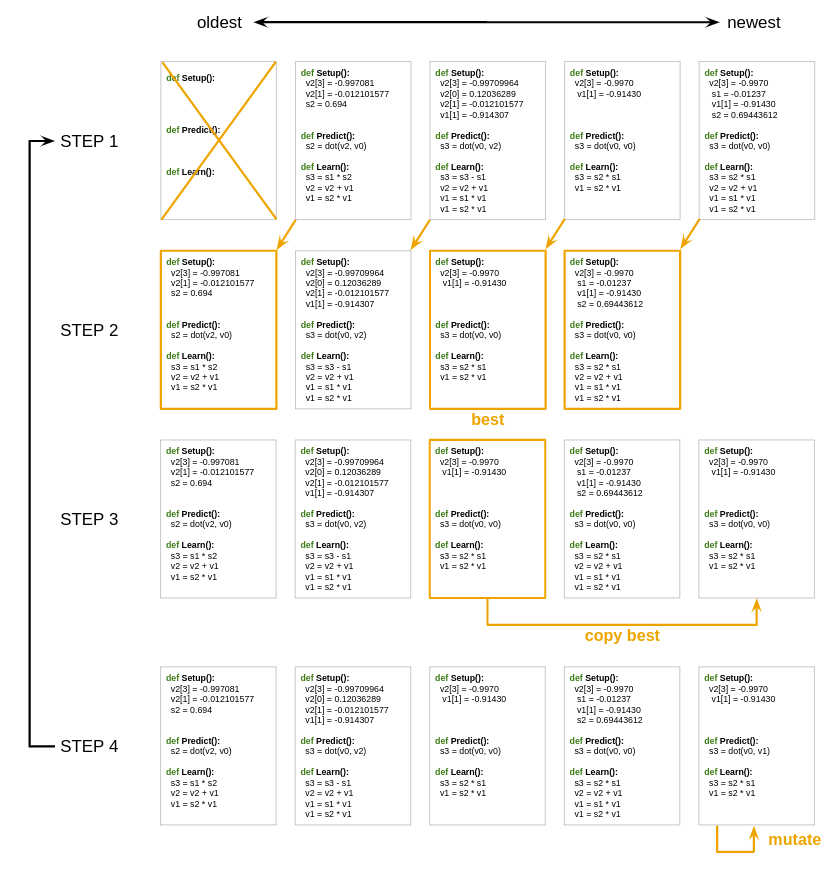
\includegraphics[width=14cm]{regularized_evolution.png}
  \caption{RE-AutoML-Zero\cite{automl_zero}の世代交代モデル. STEP1からSTEP4を繰り返すことで最適なアルゴリズムの発見を目指す. STEP1で最も古い個体を削除した後に, STEP2でトーナメント選択を行う. その後, STEP3でトーナメント選択によって選ばれた個体をコピーし, STEP4で一定確率$p_\mathrm{mutate}$で突然変異を行う. }
  \label{fig:regularized_evolution}
\end{figure}


Estebanらが提案したRE-AutoML-Zeroでは, $N_\mathrm{pop}$個のアルゴリズムをランダムに初期集団として生成した後に, Fig.\ref{fig:regularized_evolution}のSTEP1からSTEP4に示したRegularized Evolution (RE) を繰り返し行うことで, 最適なアルゴリズムの探索を行う. REでは, STEP1で最も古い個体を削除した後に, STEP2でトーナメント選択, すなわち$K( < N_\mathrm{pop})$個の個体を非復元抽出した上で最も評価値の高い個体を選択を行う. その後, STEP3でトーナメント選択によって選ばれた個体をコピーし, STEP4で一定確率$p_\mathrm{mutate}$で突然変異を行う. 集団サイズ$N_\mathrm{pop}$, トーナメントサイズ$K$, 突然変異確率$p_\mathrm{mutate}$はユーザパラメータである.


\begin{breakablealgorithm}[tbp]
  \caption{RE-AutoML-Zeroのアルゴリズム}
  \label{algorithm:re_automl_zero}
  \begin{algorithmic}[1]
    \REQUIRE タスク集合$\mathcal{T}_\mathrm{search}$, 集団サイズ$N_\mathrm{pop}$, トーナメントサイズ$K$, 突然変異確率$p_\mathrm{mutate}$, 最大評価回数$ N_\mathrm{eval}$
    \ENSURE 探索結果のアルゴリズム
    \STATE $ (P,\ \mathrm{best}) \leftarrow \mathrm{initialize}(N_\mathrm{pop})$
    \STATE $\mathrm{eval\_num} \leftarrow N_\mathrm{pop}$
    \WHILE{$\mathrm{eval\_num} < N_\mathrm{eval}$}
    \STATE $\mathrm{remove\_oldest}(P)$
    \STATE $a= \mathrm{tournament\_select}(P, K)$
    \IF{   $\mathrm{rand}(0, 1) < p_\mathrm{mutate}$}
    \STATE $\mathrm{mutate}(a)$
    \STATE $\mathrm{algorithm.fitness} \leftarrow  \mathrm{evaluate}(a, \mathcal{T}_\mathrm{search})$
    \STATE $\mathrm{eval\_num} \leftarrow \mathrm{eval\_num} + 1 $
    \IF{   $\mathrm{algorithm.fitness} > \mathrm{best.fitness} $}
    \STATE $\mathrm{best} \leftarrow a$
    \ENDIF
    \ENDIF
    \STATE $\mathrm{add}(P, a)$
    \ENDWHILE
    \RETURN best
  \end{algorithmic}
\end{breakablealgorithm}

RE-AutoML-Zeroの詳細なアルゴリズムをAlgorithm \ref{algorithm:re_automl_zero}に示す. Algorithm \ref{algorithm:re_automl_zero}の入力(Input)はタスク集合$\mathcal{T}_\mathrm{search}$, 集団サイズ$N_\mathrm{pop}$, トーナメントサイズ$K$, 突然変異確率$p_\mathrm{mutate}$, 最大評価回数$ N_\mathrm{eval}$である. また, 出力(Output)は探索結果のアルゴリズムである. Algorithm \ref{algorithm:re_automl_zero}の各行の説明を以下に示す.

\begin{description}
  \item[1行目] $\mathrm{initialize}$を用いて, アルゴリズム(個体)をランダムに$N_\mathrm{pop}$個生成した上で, 各アルゴリズムを評価を行う.  $\mathrm{initialize}(N_\mathrm{pop})$の返り値は, 生成された初期集団と初期集団内の評価値が最上位のアルゴリズム(個体)である. 初期集団内の個体は, 第\ref{subsec:problem:existing_method:mutation}項で述べる突然変異手法(2)をSetup, Predict, Learnすべてに適用することで生成する. このとき, 各関数の命令数は事前にユーザパラメータとして与える.
  \item[2行目] 評価回数のカウンターを初期集団生成分の$N_\mathrm{pop}$で初期化する.
  \item[3-15行目] 評価回数が上限を超えるまでREによる世代交代を繰り返す.
    \begin{description}
      \item[4行目] 集団$P$から最も古いアルゴリズム(個体)を除去する関数$\mathrm{remove\_oldest}(P)$を実行する.
      \item[5行目] 集団$P$からトーナメントサイズ$K$でトーナメント選択する関数$\mathrm{tournament\_select}(P, K)$を実行する. $\mathrm{tournament\_select}$の返り値は, 選択されたアルゴリズムのコピーである.
      \item[6-13行目] 一定確率$p_\mathrm{mutate}$で突然変異を行い, 評価値が改善されたらbestに反映する. ここで, $\mathrm{rand}(0, 1)$ : 0から1の範囲の実数の一様乱数を表す.
        \begin{description}
          \item[7行目] アルゴリズム$a$を突然変異させる関数$\mathrm{mutate}(a)$を実行する. 突然変異方法の詳細は第\ref{subsec:problem:existing_method:mutation}項で述べる.
          \item[8行目] タスク集合$\mathcal{T_\mathrm{search}}$に対するアルゴリズム$a$の評価値を第\ref{subsec:problem:existing_method:algorithm_eval}項に示した方法で計算する関数$\mathrm{evaluate}(\mathcal{T_\mathrm{search}}, a)$を実行し, 個体に記録する.
          \item[9行目] 評価回数をインクリメントする.
          \item[10-12行目] 突然変異した結果のアルゴリズム$a$の評価値が現状のbestを超える場合はbestに$a$を格納する.
        \end{description}
      \item[14行目] 集団$P$にアルゴリズム$a$を追加する関数$\mathrm{add}(P, a)$を実行する.
    \end{description}
  \item[16行目] bestを返却する.
\end{description}

\subsection{突然変異による個体生成}\label{subsec:problem:existing_method:mutation}

\begin{figure}
  \centering
  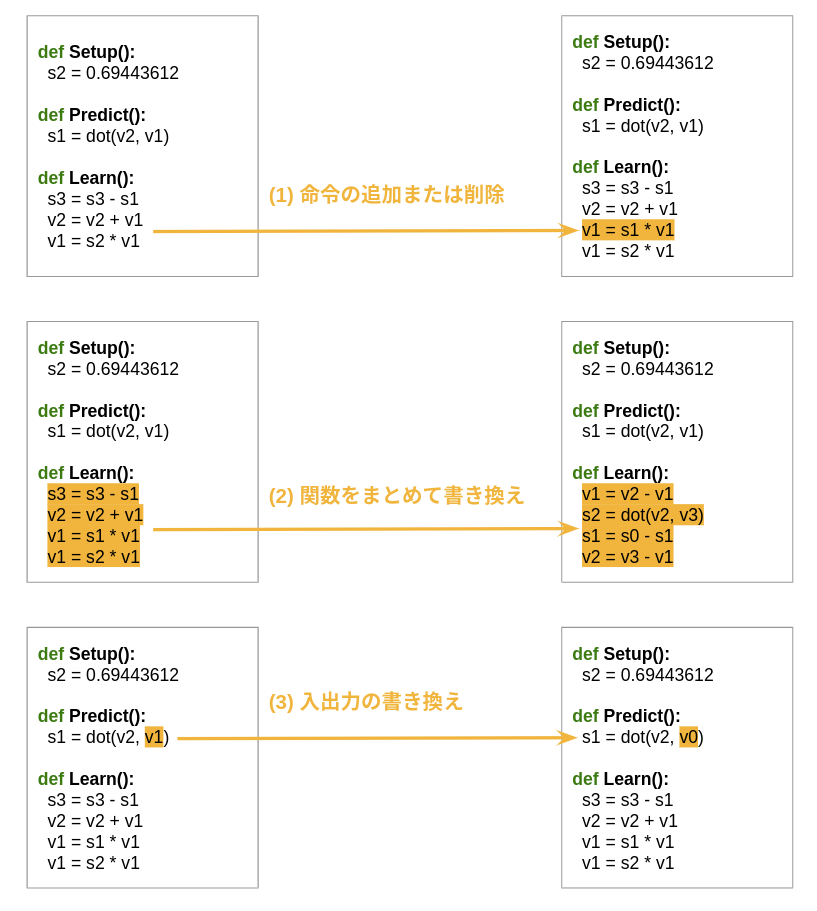
\includegraphics[width=10cm]{mutation.png}
  \caption{突然変異の種類\cite{automl_zero}. (1) アルゴリズムのSetup, Predict, Learnのいずれかをランダムに選択した上で, ランダムに命令を追加または削除する. (2) アルゴリズムのSetup, Predict, Learnのいずれかをすべてランダムな命令列で書き換える. (3) アルゴリズム内のいずれかの命令の入出力をランダムに変更する. }
  \label{fig:re_automl_zero:mutation}
\end{figure}

RE-AutoML-Zeroの突然変異は図\ref{fig:re_automl_zero:mutation}に示した3種類が存在する. それぞれの突然変異手法の以下で説明する.

\begin{enumerate}
  \renewcommand{\labelenumi}{(\arabic{enumi})}
  \item アルゴリズムの構成要素(Setup, Predict, Learn)のいずれかを一様ランダムに選択した上で, 選択された構成要素に対して命令の追加または削除を行う突然変異. 追加または削除する場所も一様ランダムに決まる.
  \item アルゴリズムの構成要素(Setup, Predict, Learn)のいずれかを, ランダムな命令列で書き換える突然変異. 命令数は元の個数と変更しない.
  \item アルゴリズムの構成要素(Setup, Predict, Learn)のいずれかを選択した上で, その構成要素内の1つの命令の入力, 出力もしくは即値のいずれかをランダムに変更する突然変異.
\end{enumerate}
\noindent
突然変異はユーザが与える制限を満たす範囲でのみ行うことができる. 具体的には, ユーザは各構成要素に含まれる命令数の下限および上限, 各構成要素に含められる命令の種類, 仮想メモリ上の変数の個数を指定することができる. そのため, (1)によってユーザが設定した構成要素の命令数の上限を超えた追加や下限を下回る削除を行ったり, (2)によって許可されていない命令を構成要素に含めることは出来ない. また, 仮想メモリ上のスカラーの変数の個数が3個と決まっている場合, すなわち$s0$から$s2$まで使える場合に, (3)で命令の入力変数として$s4$に設定することはできない.

\section{おわりに}\label{sec:problem:con}
本章では, 本研究で対象とする問題設定を明確にした上で, 既存手法であるEstebanらの手法RE-AutoML-Zeroにおけるアルゴリズムの表現方法やアルゴリズムの評価方法, 世代交代モデル, 突然変異手法について説明した.

\chapter{MGG-AutoML-Zero+AV}\label{chap:mgg_automl_zero_av}

\section{はじめに}\label{sec:mgg_automl_zero_av:intr}

本章では, 既存手法であるEstebanらの手法RE-AutoML-Zeroの問題点を指摘した上で, その問題点に対処した手法を提案する. 既存手法には世代交代モデルに関する問題点と探索空間の冗長性に関する問題があると考えられる.  提案手法では, 新たな世代交代モデルMinimal Generation Gap (MGG)を導入した上で, 妥当であるかを検証する処理(Algorithm Validation, AV)を行うことでこれらの問題点に対処する.  以下, 第\ref{sec:mgg_automl_zero_av:existing_problem}節ではRE-AutoML-Zeroの問題点の詳細, 第\ref{sec:mgg_automl_zero_av:suggest}節では問題点対処した提案手法を説明する.  本章では, 既存手法はRE-AutoML-Zero, 提案手法はMGG-AutoML-Zero+AVを指す.

\section{RE-AutoML-Zeroの問題点}\label{sec:mgg_automl_zero_av:existing_problem}

既存手法のRE-AutoML-Zeroには, 集団の多様維持および探索空間の冗長性に関する問題が存在すると考えられる. 以下では, それぞれの問題点の詳細を述べる.

\subsection{集団の多様維持に関する問題}\label{subsec:mgg_automl_zero_av:existing_problem:diversity}

既存手法のRE-AutoML-Zeroで採用されている世代交代モデルであるREは, 集団の多様性を失いやすいと考えられる. 佐藤らの論文\cite{mgg}の考察を踏まえると, REが集団の多様性を低下させる要因として, 主に以下の3点が考えられる.

\begin{enumerate}
  \item Fig.\ref{fig:regularized_evolution}のSTEP1 (Algorithm \ref{algorithm:re_automl_zero}の17行目)において, 無条件で元の集団の個体が淘汰されている点
  \item Fig.\ref{fig:regularized_evolution}のSTEP2 (Algorithm \ref{algorithm:re_automl_zero}の18行目)における複製選択で, 強い選択圧が掛かるトーナメント選択が用いられている点
  \item Fig.\ref{fig:regularized_evolution}のSTEP3およびSTEP4(Algorithm \ref{algorithm:re_automl_zero}の19行目から29行目)における生存選択で選ばれる個体が淘汰される個体と無関係である点
\end{enumerate}

\noindent
1つめは, 希少な構造を持つ個体も無条件で淘汰されることを意味しており, 多様性の低下を招くと考えられる. 2つめは, 探索序盤で得られた局所最適解に対しても選択圧が強く掛かることを意味しており, 十分な探索をする前に多様性を低下させる恐れがある. 3つめは, 淘汰される個体の形質が次世代に引き継げなくなることを意味しており, 集団の多様性を低下させる要因になると考えられる. これらの要因が引き起こす多様性の低下によって, 探索までに要す評価回数が増加したり, 局所最適解に陥りやすくなることが佐藤らの論文\cite{mgg}でも示されている.

\subsection{探索空間の冗長性に関する問題}\label{subsec:mgg_automl_zero_av:existing_problem:space}

既存手法RE-AutoML-Zeroでは, 妥当ではない機械学習アルゴリズムも探索対象としているため, 探索空間が冗長であり探索が非効率的になっていると考えられる. 以下では, 本論文における妥当な機械学習アルゴリズムの定義を述べた上で, 既存手法RE-AutoML-Zeroで探索対象となる妥当ではない機械学習アルゴリズムの例を挙げ, 探索空間に冗長性があることを説明する.

本論文において妥当な機械学習アルゴリズムとは, 以下の性質を有しているアルゴリズムのことをいう.

\begin{itemize}
  \item Predict関数の最後が$s1$への代入命令である.
  \item 予測ラベル$s1$に関する性質.
        \begin{itemize}
          \item 直前で代入された入力ベクトル$v0$に依存している.
          \item 学習対象のパラメータに依存している.
        \end{itemize}
  \item 学習対象のパラメータに関する性質
        \begin{itemize}
          \item 更新される前の自分自身に依存している.
          \item 直前に代入された正解ラベル$s0$に依存している
          \item 直前で代入された予測ラベル$s1$に依存している.
          \item 直前で代入された入力ベクトル$v0$に依存している
        \end{itemize}
\end{itemize}

\noindent
妥当な機械学習アルゴリズムの例をCode. \ref{code:valid_algorithm}に示す. Code. \ref{code:valid_algorithm}において学習対象のパラメータは$v1$のことである. 一般には, 学習対象のパラメータが格納される変数が$v1$以外であったり, 複数使われる場合が想定される. その場合であっても, 妥当な機械学習アルゴリズムは$v1$と同じ役割をする学習対象のパラメータを少なくとも1つは持つものとする.

既存手法RE-AutoML-Zeroでは, 多種多様な妥当ではない機械学習アルゴリズムが探索対象となる. RE-AutoML-Zeroで探索対象となる妥当ではない機械アルゴリズムの具体例をCode. \ref{code:invalid_algorithm_1}から\ref{code:invalid_algorithm_7}に示す. また, Table.\ref{table:invalid_algorithms}にCode. \ref{code:invalid_algorithm_1}から\ref{code:invalid_algorithm_7}のアルゴリズムが妥当ではない理由を示す.


妥当な機械学習アルゴリズムに要求される性質は, 機械学習タスクを高性能に解く上でタスクの種類に関係なく必要な性質であるため, 妥当ではない機械学習アルゴリズムが探索対象となっている既存手法の探索空間は冗長であると考えられる. RE-AutoML-Zeroにおけるアルゴリズム評価は, 第\ref{subsec:problem:existing_method:algorithm_exp}項に示したようにタスク集合$\mathcal{T}_\mathrm{search}$に含まれるすべてのタスクに対して学習と検証を行うため多くの時間を必要とする. そのため, 探索空間が冗長な既存手法では, 妥当ではない機械学習アルゴリズムに対して多くの評価が行われ, 探索効率を低下させていると考えられる.

\newpage

\begin{table}[tbp]
  \caption{既存手法RE-AutoML-Zeroで探索対象としている妥当ではない機械学習アルゴリズムの例と妥当ではない理由}
  \label{table:invalid_algorithms}
  \centering
  \begin{tabular}{c|p{10cm}}
    \hline
    具体例                                  & 妥当な機械学習アルゴリズムではない理由                                                      \\
    \hline \hline
    Code. \ref{code:invalid_algorithm_1} & Predict関数の最後の命令で予測ラベル$s1$に代入が行われていない.                                    \\
    Code. \ref{code:invalid_algorithm_2} & Predict関数の中で代入される予測ラベル$s1$の値がPredict関数実行前に代入される入力ベクトル$v0$に依存していない.       \\
    Code. \ref{code:invalid_algorithm_3} & Predict関数の中で代入される予測ラベル$s1$がLearn関数で更新されている学習対象のパラメータ$v1$に依存していない.        \\
    Code. \ref{code:invalid_algorithm_4} & Learn関数において代入される学習対象のパラメータ$v1$が代入前の自身に依存していない.                           \\
    Code. \ref{code:invalid_algorithm_5} & Learn関数において代入される学習対象のパラメータ$v1$がLearn関数の実行前に代入される正解ラベル$s0$に依存してない.        \\
    Code. \ref{code:invalid_algorithm_6} & Learn関数において代入される学習対象のパラメータ$v1$が直前のPredict関数で代入した予測ラベル$s1$に依存していない.       \\
    Code. \ref{code:invalid_algorithm_7} & Learn関数において代入される学習対象のパラメータ$v1$が直前のPredict関数の実行前に代入される入力ベクトル$v0$に依存していない. \\
    \hline
  \end{tabular}
\end{table}


\begin{multicols}{2}

  \begin{lstlisting}[caption=妥当な機械学習アルゴリズムの例,label=code:valid_algorithm]
  def Setup():
    s2 = 0.01

  def Predict():
    <@\blue{s1}@> = dot(v1, v0)

  def Learn():
    s3 = <@\green{s2}@> - s1
    s3 = s2 * s3
    v2 = s3 * v0
    v1 = v1 + v2
  \end{lstlisting}

  \columnbreak

  \begin{lstlisting}[caption=Predict関数の中で予測ラベル$s1$に代入が行われておらず\, 妥当ではないアルゴリズムの例. 妥当なアルゴリズムCode. \ref{code:valid_algorithm}との差分を赤字で示す. ,label=code:invalid_algorithm_1]
  def Setup():
    s2 = 0.01

  def Predict():
    <@\blue{s2}@> = dot(v1, v0)

  def Learn():
    s3 = s0 - s1
    s3 = s2 * s3
    v2 = s3 * v0
    v1 = v1 + v2
\end{lstlisting}
\end{multicols}

\newpage

\begin{multicols}{2}
  \begin{lstlisting}[caption=Predict関数の中で代入される予測ラベル$s1$の値がPredict関数実行前に代入される入力ベクトル$v0$に依存しておらず\, 妥当ではないアルゴリズムの例. 妥当なアルゴリズムCode. \ref{code:valid_algorithm}との差分を赤字で示す. ,label=code:invalid_algorithm_2]
    def Setup():
      s2 = 0.01

    def Predict():
      s1 = dot(v1, <@\red{v3}@>)

    def Learn():
      s3 = s0 - s1
      s3 = s2 * s3
      v2 = s3 * v0
      v1 = v1 + v2
  \end{lstlisting}

  \columnbreak

  \begin{lstlisting}[caption=Predict関数の中で代入される予測ラベル$s1$がLearn関数で更新されている学習対象のパラメータ$v1$に依存して依存しておらず\, 妥当ではないアルゴリズムの例. 妥当なアルゴリズムCode. \ref{code:valid_algorithm}との差分を赤字で示す. ,label=code:invalid_algorithm_3]
    def Setup():
      s2 = 0.01

    def Predict():
      s1 = dot(<@\red{v3}@>, v0)

    def Learn():
      s3 = s0 - s1
      s3 = s2 * s3
      v2 = s3 * v0
      v1 = v1 + v2
  \end{lstlisting}
\end{multicols}

\begin{multicols}{2}
  \begin{lstlisting}[caption=Learn関数において代入される学習対象のパラメータ$v1$が代入前の自身に依存しておらず\, 妥当ではないアルゴリズムの例. 妥当なアルゴリズムCode. \ref{code:valid_algorithm}との差分を赤字で示す. ,label=code:invalid_algorithm_4]
    def Setup():
      s2 = 0.01

    def Predict():
      s1 = dot(v1, v0)

    def Learn():
      s3 = s0 - s1
      s3 = s2 * s3
      v2 = s3 * v0
      v1 = <@\red{v0}@> + v2
  \end{lstlisting}

  \columnbreak

  \begin{lstlisting}[caption=Learn関数において代入される学習対象のパラメータ$v1$がLearn関数の実行前に代入される正解ラベル$s0$に依存しておらず\, 妥当ではないアルゴリズムの例. 妥当なアルゴリズムCode. \ref{code:valid_algorithm}との差分を赤字で示す. ,label=code:invalid_algorithm_5]
    def Setup():
      s2 = 0.01

    def Predict():
      s1 = dot(v1, v0)

    def Learn():
      s3 = <@\green{s2}@> - s1
      s3 = s2 * s3
      v2 = s3 * v0
      v1 = v1 + v2
  \end{lstlisting}
\end{multicols}

\newpage

\begin{multicols}{2}
  \begin{lstlisting}[caption=Learn関数において代入される学習対象のパラメータ$v1$が直前のPredict関数で代入した予測ラベル$s1$に依存しておらず\, 妥当ではないアルゴリズムの例. 妥当なアルゴリズムCode. \ref{code:valid_algorithm}との差分を赤字で示す. ,label=code:invalid_algorithm_6]
    def Setup():
      s2 = 0.01

    def Predict():
      s1 = dot(v1, v0)

    def Learn():
      s3 = s0 - <@\red{s2}@>
      s3 = s2 * s3
      v2 = s3 * v0
      v1 = v1 + v2
  \end{lstlisting}

  \columnbreak

  \begin{lstlisting}[caption=Learn関数において代入される学習対象のパラメータ$v1$が直前のPredict関数の実行前に代入される入力ベクトル$v0$に依存しておらず\, 妥当ではないアルゴリズムの例. 妥当なアルゴリズムCode. \ref{code:valid_algorithm}との差分を赤字で示す. ,label=code:invalid_algorithm_7]
    def Setup():
      s2 = 0.01

    def Predict():
      s1 = dot(v1, v0)

    def Learn():
      s3 = s0 - s1
      s3 = s2 * s3
      v2 = s3 * <@\red{v1}@>
      v1 = v1 + v2
  \end{lstlisting}
\end{multicols}

\section{提案手法}\label{sec:mgg_automl_zero_av:suggest}

本章では, 既存手法であるEstebanらの手法の問題点に対処した手法を提案する. 提案手法では, 既存手法のRE-AutoML-Zeroを大きく分けて2つの点で見直した.

1つめは世代交代モデルである. 第\ref{subsec:mgg_automl_zero_av:existing_problem:diversity}項で述べたように, RE-AutoML-Zeroで用いられているREは集団の多様性を失いやすい世代交代モデルであった. そこで本研究では, 佐藤らが論文\cite{mgg}の中で提案した世代交代モデルMinimal Generation Gap (MGG)を導入することで, 集団の多様性を維持しやすくなるように工夫する. 以降, RE-AutoML-Zeroの世代交代モデルをMGGに変更した手法をMGG-AutoML-Zeroと呼ぶ.

2つめは探索空間である. 第\ref{subsec:mgg_automl_zero_av:existing_problem:space}項で述べたように, RE-AutoML-Zeroでは妥当ではない機械学習アルゴリズムが探索空間に多く含まれていた. そこで我々は, 機械学習アルゴリズムとして妥当であるかを検証する処理(Algorithm Validation, AV)をアルゴリズムの生成の度に行うことで, 妥当ではない機械学習アルゴリズムを実行不可能解とする手法を提案する. 以降, MGG-AutoML-ZeroにAVを加えた手法をMGG-AutoML-Zero+AVと呼ぶ.

以下, 第\ref{subsec:mgg_automl_zero_av:suggest:mgg}項ではMGGによる集団の多様性維持の基本的な考え方と詳細, 第\ref{subsec:mgg_automl_zero_av:suggest:av}項ではAVによる探索空間の削減の基本的な考え方と詳細を述べる.

\subsection{MGGによる集団の多様性維持}\label{subsec:mgg_automl_zero_av:suggest:mgg}

本節では, \ref{subsubsec:mgg_automl_zero_av:suggest:mgg:basic}でMGGによる集団の多様性維持の基本的な考え方を述べた後で, \ref{subsubsec:mgg_automl_zero_av:suggest:mgg:detail}でMGG-AutoML-Zeroのアルゴリズムの詳細を述べる.

\subsubsection{MGG-AutoML-Zeroの基本的な考え方}\label{subsubsec:mgg_automl_zero_av:suggest:mgg:basic}

\begin{figure}[tbp]
  \centering
  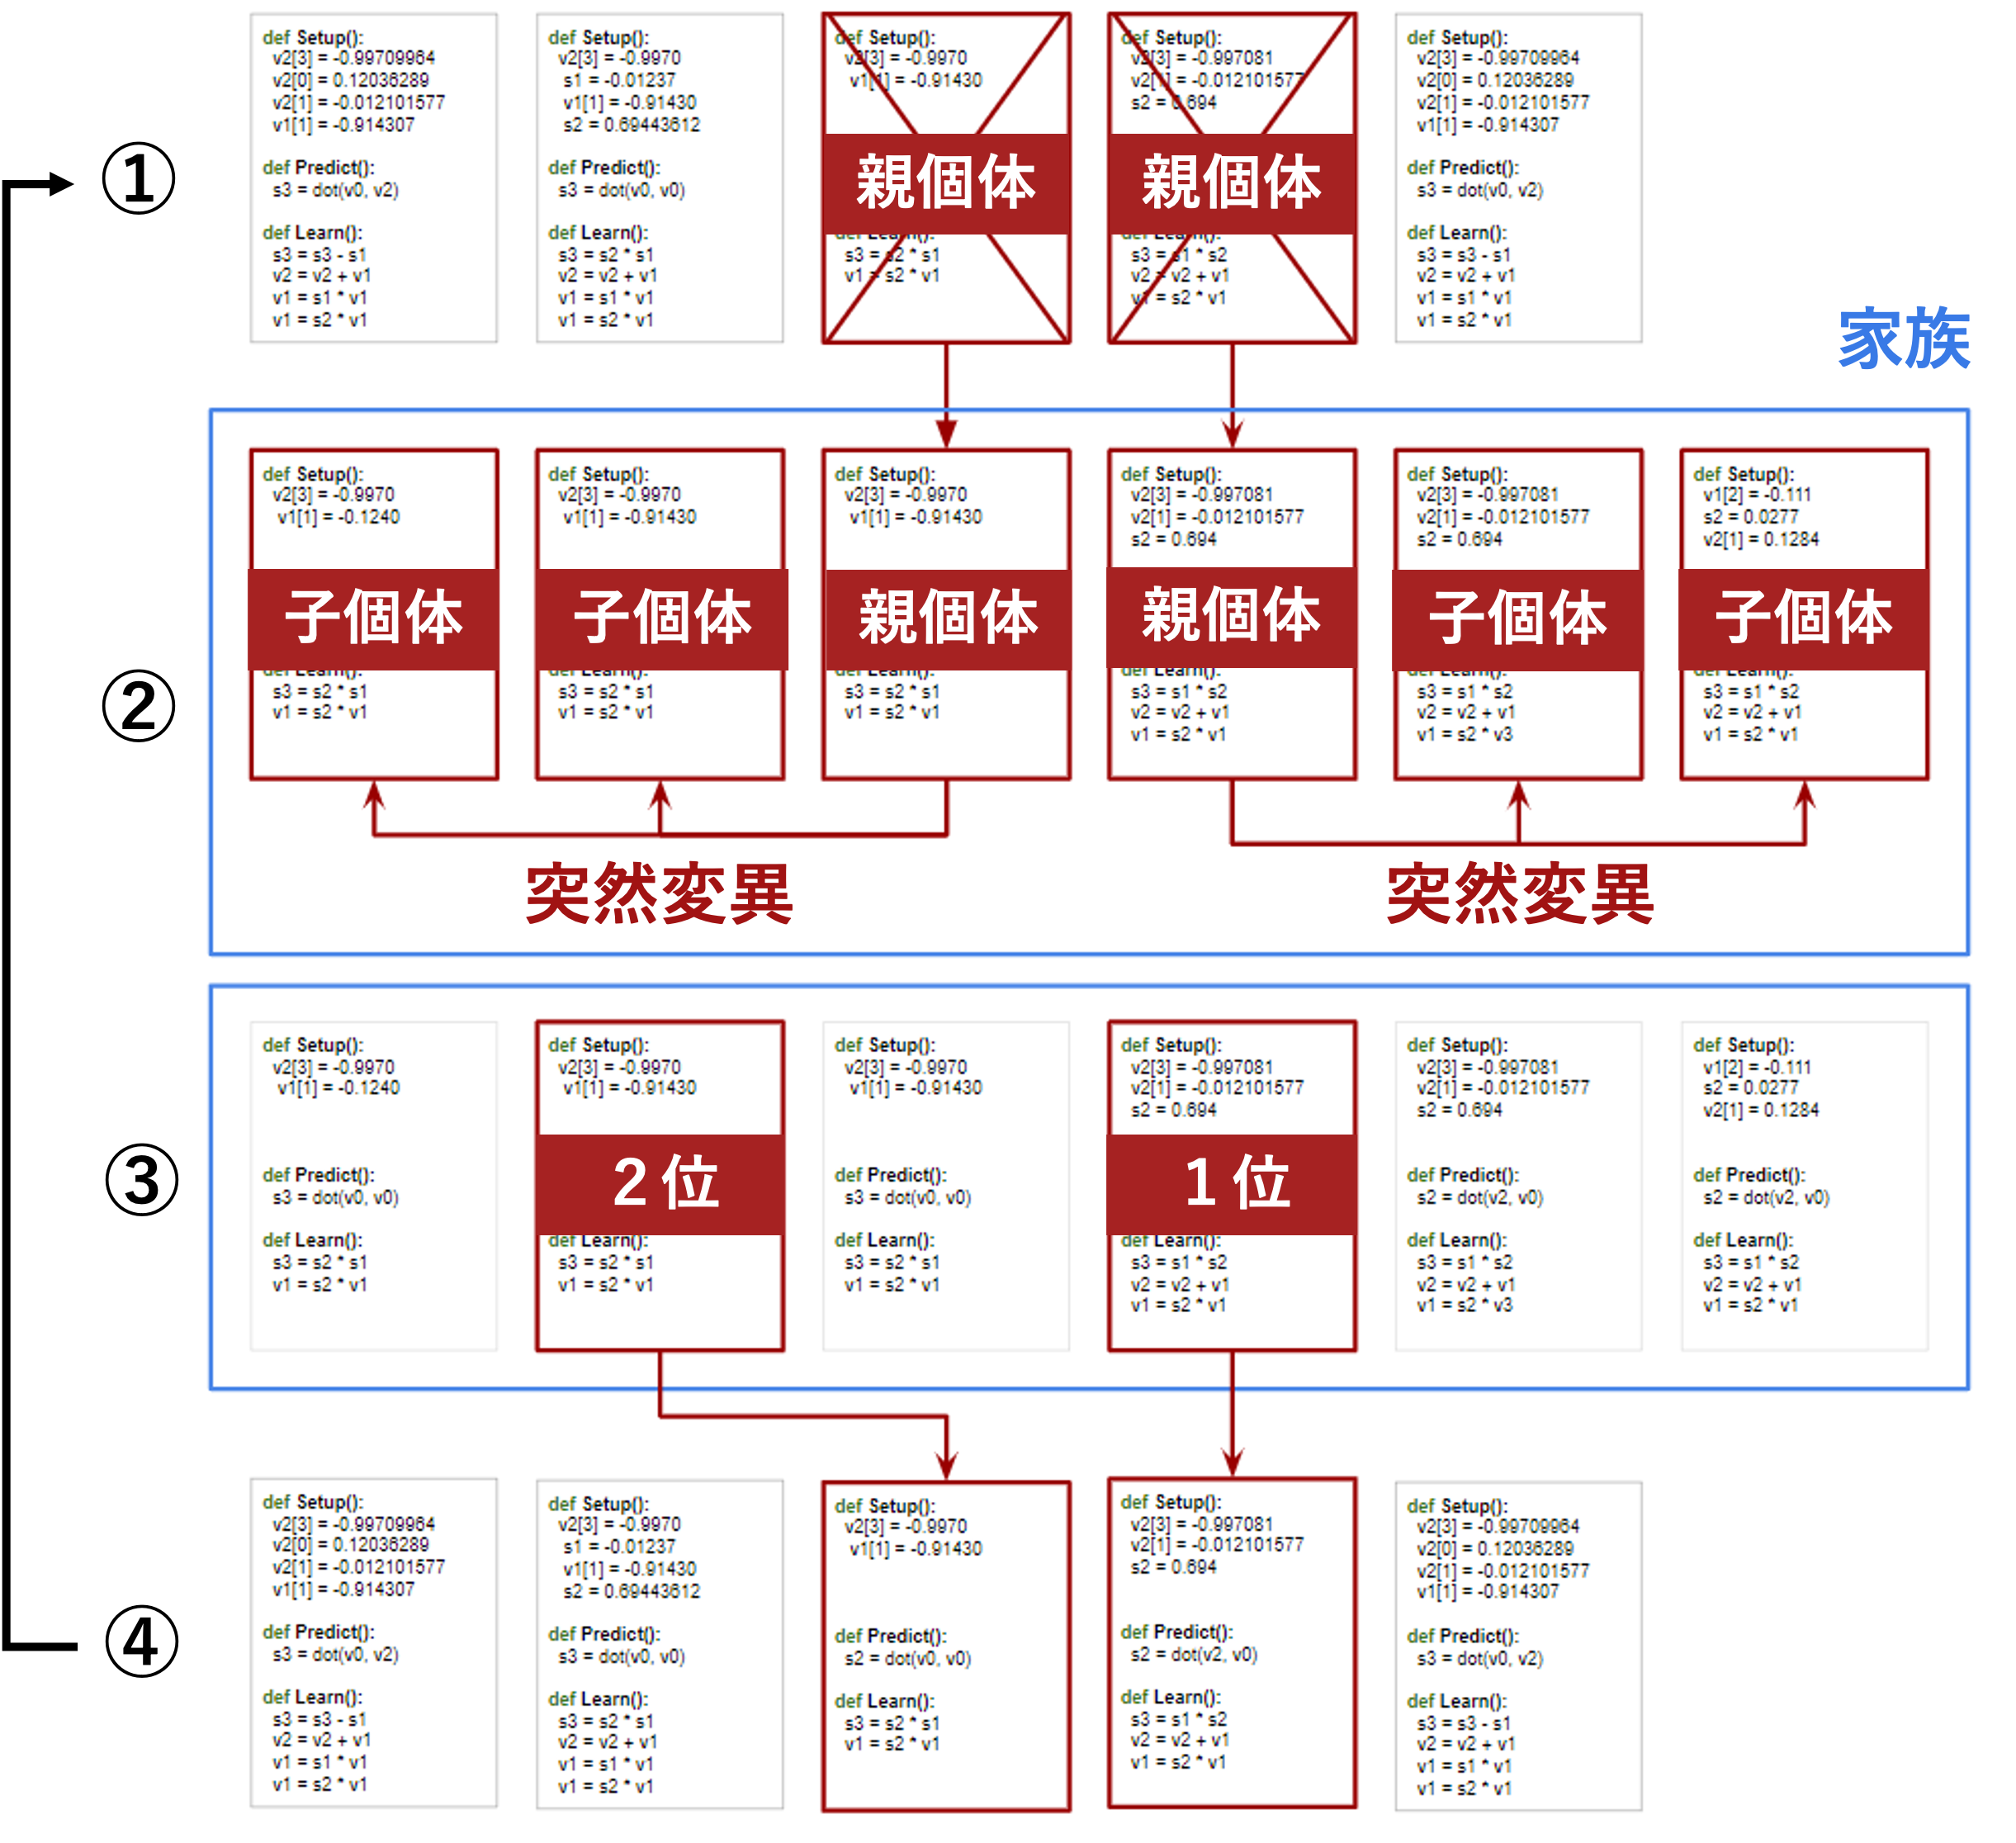
\includegraphics[width=14cm]{mgg.png}
  \caption{MGG-AutoML-Zeroの世代交代モデル. STEP1からSTEP4を繰り返す. STEP1で無作為に2つのアルゴリズム$p_a$, $p_b$を親個体として取り出し, STEP2で$p_a$を突然変異させた個体を$N_\mathrm{children} / 2$個, $p_b$を突然変異させた個体を$N_\mathrm{children} / 2$個つくり, 合計で$N_\mathrm{children}$個の子個体を生成する. その後のSTEP3,4では, 生成した$N_\mathrm{children}$個の子個体と親個体$p_a$, $p_b$の中で最も評価値が高い上位2つの個体を集団に戻す. }
  \label{fig:mgg}
\end{figure}


MGG-AutoML-Zeroでは, RE-AutoML-Zeroと同様の方法で初期集団を生成した後に, Fig.\ref{fig:mgg}に示したMGGによる世代交代を繰り返し行う. 各世代交代では, STEP1で無作為に2つのアルゴリズム$p_a$, $p_b$を親個体として取り出し, STEP2で$p_a$を突然変異させた個体を$N_\mathrm{children} / 2$個, $p_b$を突然変異させた個体を$N_\mathrm{children} / 2$個つくり, 合計で$N_\mathrm{children}$個の子個体を生成する. その後のSTEP3,4では, 生成した$N_\mathrm{children}$個の子個体と親個体$p_a$, $p_b$の中で最も評価値が高い上位2つの個体を集団に戻す. 集団サイズ$N_\mathrm{pop}$, 子個体生成数$N_\mathrm{children}$はユーザパラメータである.

RE-AutoML-ZeroからMGG-AutoML-Zeroになることで, 第\ref{subsec:mgg_automl_zero_av:existing_problem:diversity}項で述べた3つの集団の多様性を低下させる要因に対処できると考えられる. 以下に, 集団の多様性を低下させる3つの要因の内容を再掲し, MGG-AutoML-Zeroにすることで対処可能になる理由を示す.

\begin{description}
  \item[多様性低下要因1]
    \begin{description}
      \item[(内容)] RE-AutoML-Zeroでは, Fig.\ref{fig:regularized_evolution}のSTEP1 (Algorithm \ref{algorithm:re_automl_zero}の17行目)において, 無条件で元の集団の個体が淘汰されている.
      \item[(対処可能な理由)] MGG-AutoML-Zeroでは, Fig.\ref{fig:mgg}のSTEP1で淘汰される候補となった親個体も, Fig.\ref{fig:mgg}のSTEP3, 4の生存選択で集団に戻される可能性があるため, 集団内の個体が無条件で淘汰されることはない.
    \end{description}
  \item[多様性低下要因2]
    \begin{description}
      \item[(内容)] RE-AutoML-Zeroでは, Fig.\ref{fig:regularized_evolution}のSTEP2 (Algorithm \ref{algorithm:re_automl_zero}の18行目)における複製選択で, 強い選択圧が掛かるトーナメント選択が用いられている.
      \item[(対処可能な理由)] MGG-AutoML-Zeroでは, Fig.\ref{fig:mgg}のSTEP1で無作為に複製選択するため, 複製選択で強い選択圧がかかることはない.
    \end{description}
  \item[多様性低下要因3]
    \begin{description}
      \item[(内容)] RE-AutoML-Zeroでは, Fig.\ref{fig:regularized_evolution}のSTEP3およびSTEP4(Algorithm \ref{algorithm:re_automl_zero}の19行目から29行目)における生存選択で選ばれる個体が淘汰される個体と無関係である.
      \item[(対処可能な理由)] MGG-AutoML-Zeroでは, Fig.\ref{fig:mgg}のSTEP3, 4における生存選択で選ばれる個体が, 淘汰される候補である親個体の家族に限定されている.
    \end{description}
\end{description}

佐藤らの論文\cite{mgg}のMGGにおける生存選択は, 子個体と親個体の中から最上位の個体とルーレット選択で選ばれた個体を取り出すことで行っていたが, 本研究のMGGの生存選択では, 最も評価値が高い上位2つを取り出すことで行う. 佐藤らの論文\cite{mgg}の対象問題では, 生成される子個体の評価値が親個体よりも改善される可能性が高い. 一方, 本研究で生成される子個体は突然変異オペレータのランダム性が高く, 親個体より評価値が高い子個体が得られる可能性が低い. 故に, ルーレット選択をしてしまうと, 評価値が悪い個体が数によって選ばれてしまい, 進化が滞ってしまうと考えられる.

\subsubsection{MGG-AutoML-Zeroの詳細なアルゴリズム}\label{subsubsec:mgg_automl_zero_av:suggest:mgg:detail}

MGG-AutoML-Zeroの詳細なアルゴリズムをAlgorithm \ref{algorithm:mgg_automl_zero}に示す. Algorithm \ref{algorithm:mgg_automl_zero}の入力(Input)はタスク集合$\mathcal{T}_\mathrm{search}$, 集団サイズ$N_\mathrm{pop}$, 子個体生成数$N_\mathrm{children}$, 最大評価回数$ N_\mathrm{eval}$である. また, 出力(Output)は探索結果のアルゴリズムである. Algorithm \ref{algorithm:mgg_automl_zero}の各行の説明を以下に示す.

\begin{description}
  \item[1行目] RE-AutoML-Zeroと同様の方法で初期集団を生成して評価を行う.
  \item[2行目] 評価回数のカウンターを初期集団生成分の$N_\mathrm{pop}$で初期化する.
  \item[3-41行目] 評価回数が上限を超えるまでMGGによる世代交代を繰り返す.
    \begin{description}
      \item[4-5行目] 集団$P$からランダムにアルゴリズム(個体)を非復元抽出する関数$\mathrm{randomly\_remove}(P)$を用いて親個体を2つ選択する.
      \item[6-12行目] 2つの親子体のうち評価値が高い方を$\mathrm{best}1$, 低い方を$\mathrm{best}2$に設定する. $\mathrm{best}1$と$\mathrm{best}2$は, 最後に集団に戻す対象となるアルゴリズムを格納する用の変数である.
      \item[13行目] 子個体の生成indexを0で初期化する.
      \item[14-35行目] 子個体を$N_\mathrm{children}$個生成する用のループを実行する.
        \begin{description}
          \item[15-19行目] $\mathrm{child\_index} < N_\mathrm{children} / 2$の場合は$\mathrm{child}$に$\mathrm{parent}1$をコピーし, それ以外の場合は$\mathrm{child}$に$\mathrm{parent}2$をコピーする. これにより, それぞれの親個体から$N_\mathrm{children} / 2$個ずつ個体を生成することが可能となる.
          \item[20行目] 親個体いずれかのコピーである$\mathrm{child}$を突然変異させる. 突然変異に使う関数$\mathrm{mutate}$はRE-AutoML-Zeroと同じである.
          \item[21行目] RE-AutoML-Zeroと同様の方法で, $\mathcal{T}_\mathrm{search}$に対するアルゴリズム$\mathrm{child}$の評価を行う.
          \item[22行目] 評価回数をインクリメントする.
          \item[23-30行目] 子個体$\mathrm{child}$の評価値が$\mathrm{best}2$以上である場合は, 適切に順位を更新する.
          \item[31-33行目] この時点で評価回数が上限を超えた場合は, 子個体が所定の個数生成されていなくても強制的に子個体生成のループから抜ける.
          \item[34行目] 子個体の生成indexをインクリメントする.
        \end{description}
      \item[36-37行目] 集団$P$にアルゴリズム$a$を追加する関数$\mathrm{add}(P, a)$を用いて, $\mathrm{best}1$と$\mathrm{best}2$を集団に追加する.
      \item[38-40行目] アルゴリズム$\mathrm{best}1$の評価値が現状のbestを超える場合はbestに$\mathrm{best}1$を格納する
    \end{description}
  \item[42行目] bestを返却する.
\end{description}

\begin{breakablealgorithm}
  \caption{AutoML-Zero+MGGのアルゴリズム}
  \label{algorithm:mgg_automl_zero}
  \begin{algorithmic}[1]
    \REQUIRE 集団サイズ$N_\mathrm{pop}$, 子個体生成数$N_\mathrm{children}$, 最大評価回数$ N_\mathrm{eval}$
    \ENSURE 探索結果のアルゴリズム
    \STATE $ (P,\ \mathrm{best}) \leftarrow \mathrm{initialize}(N_\mathrm{pop})$
    \STATE $\mathrm{eval\_num} \leftarrow N_\mathrm{pop}$
    \WHILE{$\mathrm{eval\_num} < N_\mathrm{eval}$}
    \STATE $\mathrm{parent}1 = \mathrm{randomly\_remove}(P)$
    \STATE $\mathrm{parent}2 = \mathrm{randomly\_remove}(P)$
    \IF{   $\mathrm{parent}1.\mathrm{fitness} > \mathrm{parent}2.\mathrm{fitness} $}
    \STATE $ \mathrm{best}1 \leftarrow \mathrm{parent}1 $
    \STATE $ \mathrm{best}2 \leftarrow \mathrm{parent}2 $
    \ELSE
    \STATE $ \mathrm{best}1 \leftarrow \mathrm{parent}2 $
    \STATE $ \mathrm{best}2 \leftarrow \mathrm{parent}1 $
    \ENDIF
    \STATE $ \mathrm{child\_index} \leftarrow 0 $
    \WHILE{$ \mathrm{child\_index} < N_\mathrm{children}$}
    \IF{   $\mathrm{child\_index} < N_\mathrm{children} / 2  $}
    \STATE $ \mathrm{child} \leftarrow \mathrm{copy}(\mathrm{parent}1) $
    \ELSE
    \STATE $ \mathrm{child} \leftarrow \mathrm{copy}(\mathrm{parent}2) $
    \ENDIF
    \STATE $\mathrm{mutate}(\mathrm{child}) $
    \STATE $\mathrm{child}.\mathrm{fitness} \leftarrow \mathrm{evaluate}(\mathrm{child}) $
    \STATE $\mathrm{eval\_num} \leftarrow \mathrm{eval\_num} + 1 $
    \IF{   $\mathrm{child}.\mathrm{fitness} \geq \mathrm{best}2.\mathrm{fitness}$}
    \IF{   $\mathrm{child}.\mathrm{fitness} \geq \mathrm{best}1.\mathrm{fitness}$}
    \STATE $ \mathrm{best}2 \leftarrow \mathrm{best}1 $
    \STATE $ \mathrm{best}1 \leftarrow \mathrm{child} $
    \ELSE
    \STATE $ \mathrm{best}2 \leftarrow \mathrm{child} $
    \ENDIF
    \ENDIF
    \IF{   $\mathrm{eval\_num} \geq  N_\mathrm{eval}$}
    \STATE $ \mathrm{break} $
    \ENDIF
    \STATE $ \mathrm{child\_index} \leftarrow \mathrm{child\_index} + 1 $
    \ENDWHILE
    \STATE $\mathrm{add}(P, \mathrm{best}1)$
    \STATE $\mathrm{add}(P, \mathrm{best}2)$
    \IF{   $\mathrm{best1}.\mathrm{fitness} > \mathrm{best}.\mathrm{fitness}$}
    \STATE $ \mathrm{best} \leftarrow \mathrm{best}1 $
    \ENDIF
    \ENDWHILE
    \RETURN best
  \end{algorithmic}
\end{breakablealgorithm}

\subsection{AVによる探索空間の削減}\label{subsec:mgg_automl_zero_av:suggest:av}

本節では, AVによる探索空間の削減の基本的な考え方, AVを導入するにあたって必要となる依存関係解析, AVの詳細なアルゴリズムを述べる. 以下, \ref{subsubsec:mgg_automl_zero_av:suggest:av:basic}ではAVの基本的な考え方, \ref{subsubsec:mgg_automl_zero_av:suggest:av:deps_detail}では依存関係解析の詳細なアルゴリズム, \ref{subsubsec:mgg_automl_zero_av:suggest:av:detail}ではAVの詳細なアルゴリズムについて述べる.

\subsubsection{AVの基本的な考え方}\label{subsubsec:mgg_automl_zero_av:suggest:av:basic}

アルゴリズムの検証(AV)を導入した手法では, Fig.\ref{fig:av}に示したように妥当な機械学習アルゴリズム(個体)が生成されるまで個体の生成を繰り返す. これによって, 妥当ではない機械学習アルゴリズムに対して, 時間のかかるアルゴリズムの評価を行わず, 実行不可能解とすることが可能となる. MGG-AutoML-Zero+AVの場合は, 初期集団の各個体を生成する時および突然変異で子個体を生成する時にFig.\ref{fig:av}の処理が行われることになる. ただし, 妥当ではないアルゴリズムは集団サイズや子個体の生成数には含めない. つまりMGG-AutoML-Zero+AVにおいて, 集団は$N_\mathrm{pop}$個の妥当な機械学習アルゴリズムであり, 子個体生成では毎回$N_\mathrm{children}$個の妥当な機械学習アルゴリズムが生成される.

\begin{figure}
  \centering
  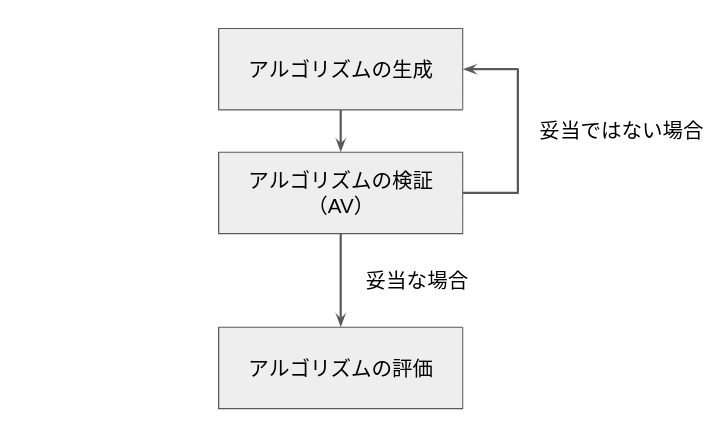
\includegraphics[width=10cm]{av.png}
  \caption{アルゴリズムの検証を導入した場合のアルゴリズムの生成から評価までの流れ. 妥当なアルゴリズムが生成されるまで生成を繰り返すことで, 妥当なアルゴリズム以外は評価が行われない. }
  \label{fig:av}
\end{figure}

AVでは, 機械学習アルゴリズムとして妥当性を以下の検証によって確認する.
\begin{itemize}
  \item Predict関数の最後がs1への代入命令であることの検証(Predict Function Validation, PFV).
  \item 予測ラベル$s1$の依存関係の検証(Prediction Label Validation, PLV)
        \begin{itemize}
          \item $\mathrm{PLV}_{v0}$: 直前で代入された入力ベクトル$v0$に依存していることの検証.
          \item $\mathrm{PLV}_\mathrm{LP}$: 学習対象のパラメータに依存していることの検証.
        \end{itemize}
  \item 学習対象のパラメータの依存関係の検証(Learning Parameter Validation, LPV)
        \begin{itemize}
          \item $\mathrm{LPV}_\mathrm{prev}$: 更新される前の自分自身に依存していることの検証.
          \item $\mathrm{LPV}_{s1}$: 直前に代入された正解ラベル$s0$に依存していることの検証.
          \item $\mathrm{LPV}_{s0}$: 直前で代入された予測ラベル$s1$に依存していることの検証.
          \item $\mathrm{LPV}_{v0}$: 直前で代入された入力ベクトル$v0$に依存していることの検証. ただし, $s1$を介した依存は含まれない.
        \end{itemize}
\end{itemize}

\begin{table}[tbp]
  \caption{AVによって実行不可能解になる具体例と制約を受ける検証の名称. 制約を受ける検証の名称は複数存在しても1つしか記載していない. }
  \label{table:invalid_algorithms_av}
  \centering
  \begin{tabular}{c|c}
    \hline
    具体例                                  & 制約を受ける検証の名称                  \\
    \hline \hline
    Code. \ref{code:invalid_algorithm_1} & PFV                          \\
    Code. \ref{code:invalid_algorithm_2} & $\mathrm{PLV}_{v0}$          \\
    Code. \ref{code:invalid_algorithm_3} & $\mathrm{PLV}_\mathrm{LP}$   \\
    Code. \ref{code:invalid_algorithm_4} & $\mathrm{LPV}_\mathrm{prev}$ \\
    Code. \ref{code:invalid_algorithm_5} & $\mathrm{LPV}_{v0}$          \\
    Code. \ref{code:invalid_algorithm_6} & $\mathrm{LPV}_{s1}$          \\
    Code. \ref{code:invalid_algorithm_7} & $\mathrm{LPV}_{v0}$          \\
    \hline
  \end{tabular}
\end{table}

\noindent
各検証はすべて第\ref{subsec:mgg_automl_zero_av:existing_problem:space}項で述べた妥当な機械学習アルゴリズムが持つ性質と1対1に対応している. AVの導入によって, 妥当ではない機械学習アルゴリズムの例として示したCode. \ref{code:invalid_algorithm_1}からCode. \ref{code:invalid_algorithm_7}はすべて実行不可能解となる. 具体的には, Table.\ref{table:invalid_algorithms_av}に示した対応関係で実行不可能解になる.

\subsubsection{依存関係解析の詳細なアルゴリズム}\label{subsubsec:mgg_automl_zero_av:suggest:av:deps_detail}

本項では, AVの導入にあたって必要となる依存関係解析の詳細なアルゴリズムについて説明する. 依存関係解析では, 命令列$F = (\mathrm{instr}_1, \mathrm{instr}_2, \cdots, \mathrm{instr}_n)$と解析対象の変数の集合$V = \left\{\mathrm{var}1, \mathrm{var}2, \cdots\right\}$が与えられた時に, $F$実行後の$\mathrm{var}1, \mathrm{var}2, \cdots$の値に影響を与える$F$実行前の変数の集合$D(F, V)$を求める. ここで, $F$はSetup, Predict, Learn等の命令列であり, $V$にはスカラー変数$s1,s2,\cdots$, ベクトル変数$v1,v2,\cdots$, 行列変数$m1,m2,\cdots$の一部が要素として含まれる. 例えば, Code. \ref{code:valid_algorithm}においては, $D\left(\mathrm{Learn}, \{ v1 \} \right) = \{ s0,\ s1,\ s2,\ v0,\ v1 \}$である. 実際, Learn実行前における$ s0,\ s1,\ s2,\ v0,\ v1 $のいずれかの値が変わると, Learn実行後の$v1$の値が変化する. これに対し, Learn実行前における$ s0,\ s1,\ s2,\ v0,\ v1 $以外の変数の値, 例えば$v2$が変わったとしても, Learn実行後の$v1$の値は変化ない.

依存関係解析は命令列を後ろから解析していくことで行うことができる. 実際, $D_i = D((\mathrm{instr}_i, \mathrm{instr}_{i+1}, \cdots, \mathrm{instr}_n), V)$,  $D_{n+1} = V$とすれば, $D_i$は$1 \le i \le n$の範囲で次の漸化式を満たす.
\begin{eqnarray}
  D_i=
  \left\{
  \begin{array}{ll}
    D_i = D_{i+1}                                                                                                  & \mathrm{output}(\mathrm{instr}_i) \not\in D_{i+1} \\
    D_i = \left(D_{i+1} \setminus {\mathrm{output}(\mathrm{instr}_i)}\right) \cup \mathrm{input}(\mathrm{instr}_i) & \mathrm{output}(\mathrm{instr}_i) \in D_{i+1}
  \end{array}
  \right.
  \label{fml:deps_recurrence}
\end{eqnarray}

\noindent
ここで, $\mathrm{output}(\mathrm{instr}_i)$は命令$\mathrm{instr}_i$の出力変数を返す関数であり, $\mathrm{input}(\mathrm{instr}_i)$は$\mathrm{instr}_i$の入力変数の集合を返す関数である.

式\ref{fml:deps_recurrence}の漸化式を用いた依存関係解析の詳細なアルゴリズムをAlgorithm \ref{algorithm:deps}に示す. Algorithm \ref{algorithm:deps}の入力(Input)は命令列$F$と解析対象の変数の集合$V$であり, 出力(Output)は$D(F, V)$である. Algorithm \ref{algorithm:deps}の各行の説明を以下に示す.

\begin{description}
  \item[1行目] $D_i$を$D_{n+1} = V$で初期化する.
  \item[2行目] $i$を$n$で初期化する.
  \item[3-10行目] 命令列の後ろから順番に解析を行う. 各ループの中では$D_i$を漸化式に基づいて更新した上で, $i$をデクリメントする.
    \begin{description}
      \item[4行目] $\mathrm{instr}_i$の出力先変数を取得し, $o$に格納する.
      \item[5-8行目] 式\ref{fml:deps_recurrence}の漸化式に従って更新をする.
      \item[9行目] $i$をデクリメントする.
    \end{description}
  \item[11行目] $D_1 = D(F,V)$を返却する.
\end{description}

\begin{breakablealgorithm}
  \caption{依存関係解析のアルゴリズム}
  \label{algorithm:deps}
  \begin{algorithmic}[1]
    \REQUIRE $F = (\mathrm{instr}_1, \mathrm{instr}_2, \cdots, \mathrm{instr}_n)$: 命令列, $V = \left\{\mathrm{var}1, \mathrm{var}2, \cdots\right\}$: 解析対象の変数の集合
    \ENSURE $D\left(F, V \right)$: 命令列$F$実行後に$\mathrm{var}1, \mathrm{var}2, \cdots$に格納されている値が依存している$F$実行前の変数の集合
    \STATE $D_i \leftarrow V $
    \STATE $ i \leftarrow n$
    \WHILE {$ i > 0 $}
    \STATE $ o \leftarrow \mathrm{output}(\mathrm{instr}_i) $
    \IF{ $ o \in D_i$ }
    \STATE $ D_i \leftarrow D_i \setminus \{ o \}$
    \STATE $ D_i \leftarrow D_i \cup \mathrm{input}(\mathrm{instr}_i) $
    \ENDIF
    \STATE $ i \leftarrow i - 1$
    \ENDWHILE
    \RETURN $D$
  \end{algorithmic}
\end{breakablealgorithm}

\subsubsection{AVの詳細なアルゴリズム}\label{subsubsec:mgg_automl_zero_av:suggest:av:detail}

アルゴリズムは, Setup, v0への代入, 1回目のPredict, s0への代入, Learn, v0への代入, 2回目のPredictという順で実行されるため, AVでは2回目のPredict実行後の$s1$の依存関係を実行の逆順で解析していくことで検証を行う. AVの詳細なアルゴリズムをAlgorithm \ref{algorithm:av}に示す. Algorithm \ref{algorithm:av}の入力(Input)は検証対象のアルゴリズムであり, 出力(Output)は検証対象のアルゴリズムが妥当な機械学習アルゴリズムであるかの真偽である. Algorithm \ref{algorithm:av}の各行の説明を以下に示す.

\begin{description}
  \item[1-3行目] PFV: Predict関数の最後がs1への代入命令であることを検証する. ここで, $\mathrm{Predict}_\mathrm{last}$はPredict関数の最後の命令を意味する.
  \item[4行目] Predict関数実行前の変数のうち, 予測ラベル$s1$の算出に影響を与える変数をすべて求めて, $D_{\mathrm{Predict},s1}$に格納する.
  \item[5-7行目] $\mathrm{PLV}_{v0}$: $s1$が直前で代入された入力ベクトル$v0$に依存していることを検証する.
  \item[8行目] Predict関数の直前に$v0$への入力ベクトルの代入が存在するため, $D_{\mathrm{Predict},s1}$から$v0$を除外する.
  \item[9行目] 学習対象のパラメータが存在するかを表すフラグ$\mathrm{learning\_param\_existence}$をfalseで初期化する.
  \item[10-28行目] $D_{\mathrm{Predict},s1}$内に学習対象のパラメータを表す変数として適切なものが存在するかを検証する. 各ループでは, 候補$c \in D_{\mathrm{Predict},s1}$に対して, 学習対象のパラメータに関する検証(LPV)を行う. 検証の結果, 学習対象のパラメータとして不適切であると判断された場合は, 当該候補の解析を終了し次の候補の解析に進む.
    \begin{description}
      \item[11行目] Learn関数実行前の変数のうち, 学習対象のパラメータ候補である$c$の算出に影響を与える変数をすべて求めて, $D_{\mathrm{Learn}, c}$に格納する.
      \item[12-14行目] $\mathrm{LPV}_\mathrm{prev}$: 学習対象のパラメータの候補$c$が更新される前の自分自身に依存していることを検証する.
      \item[15-17行目] $\mathrm{LPV}_{s0}$: 学習対象のパラメータの候補$c$が直前に代入された正解ラベル$s0$に依存していることを検証する.
      \item[18-20行目] $\mathrm{LPV}_{s1}$: 学習対象のパラメータの候補$c$が直前に代入された予測ラベル$s1$に依存していることを検証する.
      \item[21行目] Learn関数の直前に$s0$への正解ラベルの代入が存在するため, $D_{\mathrm{Learn}, c}$から$s0$を除外する. また, 学習対象のパラメータが入力ベクトル$v0$に依存しているかを検証する際は, $s1$を介した間接的な依存は許さないため, $D_{\mathrm{Learn}, c}$から$s1$も除外する.
      \item[22行目] Predict関数実行前の変数のうち, 学習対象のパラメータ候補である$c$の算出に影響を与える変数をすべて求めて, $D_{\mathrm{Predict}, \mathrm{Learn}, c}$に格納する.
      \item[23-25行目] $\mathrm{LPV}_{v0}$: 学習対象のパラメータの候補$c$が直前で代入された入力ベクトル$v0$に依存していることを検証する.
      \item[26-27行目] $\mathrm{LPV}_{v0}$: この行に到達することは, すべての学習対象のパラメータに関する検証に通ったことを意味するので, 学習対象のパラメータが存在するかを表すフラグ$\mathrm{learning\_param\_existence}$をtrueにした上でループから抜ける.
      \item[19-31行目] $\mathrm{PLV}_\mathrm{LP}$: $\mathrm{learning\_param\_existence}$がfalseである場合は, $s1$が依存している変数の集合$D_{\mathrm{Predict},s1}$に学習対象のパラメータが含まれていないことを意味するのでfalseを返却する.
    \end{description}
\end{description}

\begin{breakablealgorithm}
  \caption{AVのアルゴリズム}
  \label{algorithm:av}
  \begin{algorithmic}[1]
    \REQUIRE $(\mathrm{Setup}, \mathrm{Predict}, \mathrm{Learn})$: 検証対象のアルゴリズム
    \ENSURE 検証対象のアルゴリズムが妥当であるかの真偽
    \IF {$\mathrm{output}(\mathrm{Predict}_\mathrm{last}) \neq s1 $}
    \RETURN false
    \ENDIF
    \STATE $D_{\mathrm{Predict},s1} \leftarrow D\left(\mathrm{Predict}, \{ s1 \}\right)$
    \IF {$ v_0 \not\in D_{\mathrm{Predict},s1} $}
    \RETURN false
    \ENDIF
    \STATE $D_{\mathrm{Predict},s1} \leftarrow D_{\mathrm{Predict},s1} \setminus \{v_0\}$
    \STATE $\mathrm{learning\_param\_existence} \leftarrow \mathrm{false}$
    \FORALL {$ c \in D_{\mathrm{Predict},s1}$ }
    \STATE $D_{\mathrm{Learn}, c} \leftarrow D\left(\mathrm{Learn}, \{ c \}\right) $
    \IF {$ c \not\in D_{\mathrm{Learn}, c}  $}
    \STATE continue
    \ENDIF
    \IF {$ s_0 \not\in D_{\mathrm{Learn}, c}  $}
    \STATE continue
    \ENDIF
    \IF {$ s_1 \not\in D_{\mathrm{Learn}, c}  $}
    \STATE continue
    \ENDIF
    \STATE $D_{\mathrm{Learn}, c} \leftarrow D_{\mathrm{Learn}, c} \setminus \{s_0, s1\}$
    \STATE $D_{\mathrm{Predict}, \mathrm{Learn}, c} \leftarrow D\left(\mathrm{Predict}, D_{\mathrm{Learn}, c} \right)$
    \IF {$ v_0 \not\in D_{\mathrm{Predict}, \mathrm{Learn}, c} $}
    \STATE continue
    \ENDIF
    \STATE $\mathrm{learning\_param\_existence} \leftarrow \mathrm{true}$
    \STATE break
    \ENDFOR
    \IF {!$\mathrm{learning\_param\_existence}$}
    \RETURN false
    \ENDIF
    \RETURN true
  \end{algorithmic}
\end{breakablealgorithm}

\section{実験}\label{sec:mgg_automl_zero_av:exp}

本節では, 既存手法のRE-AutoML-Zeroと提案手法のMGG-AutoML-Zero+AVの性能を比較するための線形回帰アルゴリズムの探索実験について述べる. 以下, 第\ref{mgg_automl_zero_av:exp:purpose}項では実験の目的, 第\ref{mgg_automl_zero_av:exp:comparison}項では比較手法, 第\ref{mgg_automl_zero_av:exp:problem}項ではベンチマーク問題, 第\ref{mgg_automl_zero_av:exp:eval}項では評価基準, 第\ref{mgg_automl_zero_av:exp:setting}項では実験設定,第\ref{mgg_automl_zero_av:exp:result}項では実験結果について述べる.

\subsection{目的}\label{mgg_automl_zero_av:exp:purpose}

本実験の目的は, 線形回帰アルゴリズムの探索問題において, 既存手法であるEstebanらの手法RE-AutoML-Zeroに比べて, MGGによる世代交代とアルゴリズムの検証を加えた提案手法MGG-AutoML-Zero+AVが, 成功率および評価回数の観点で優れていることを確認することである.

\subsection{比較手法}\label{mgg_automl_zero_av:exp:comparison}

本実験では, 世代交代モデルとしてREを用いたEstebanらの手法RE-AutoML-Zeroと本論文の提案手法であるMGG-AutoML-Zero+AVを比較する.

\subsection{ベンチマーク問題}\label{mgg_automl_zero_av:exp:problem}

本実験では, 線形回帰のアルゴリズムが探索の対象であるため, $\mathcal{T}_\mathrm{search}$内の各タスク$T^{(i)}(i \in \mathbb{N},\ 1 \le i \le 10)$を以下の式で表される線形回帰問題とする.

$$
  T^{(i)} = \left\{(\bm{x}^{(i)}_j, y^{(i)}_j) \ |\ \bm{x}^{(i)}_j \sim \bm{N}(0, 1),\ y^{(i)}_j = \bm{w}_i \cdot \bm{x}^{(i)}_j,\ \bm{w}_i \sim \bm{N}(0, 1),\ j \in \mathbb{N},\ 1 \le j \le 100 \right\}
$$

\noindent
ここで, $\bm{v} \sim \bm{N}(0, 1)$は$\bm{v}$の各要素が平均$0$, 標準偏差$1$の正規乱数に従うことを意味する. 線型回帰の問題の次元$\dim(\bm{x}^{(i)}_j) = \dim(\bm{w}_i)$は$4$に設定した. タスク$T^{(i)}$のデータのうち, 100件を学習データ$D^{(i)}_\mathrm{train}$とし, 残りの100件を検証用データ$D^{(i)}_\mathrm{valid}$とする. $\bm{w}_i$はタスク$T^{(i)}$ごとに設定されるため, 10件の異なる勾配に従う線形回帰のデータセットがタスクとして与えられる点に注意されたい.

本実験では, $\mathcal{T}_\mathrm{search}$を使って探索した結果得られたアルゴリズム$\hat{a}$が$\mathcal{T}_\mathrm{search}$にオーバーフィッティングしていないことを確認するために, $\mathcal{T}_\mathrm{search}$と独立に生成されたタスク集合$\mathcal{T}_\mathrm{eval}$で$\hat{a}$を評価する. $\mathcal{T}_\mathrm{eval}$の生成方法は$\mathcal{T}_\mathrm{search}$とほぼ同じだが, $\ 1 \le i \le 100$, $\ 1 \le j \le 1100$, $\left| D^{(i)}_\mathrm{train} \right| = 1000$, $\left| D^{(i)}_\mathrm{valid} \right| = 100$となる点が異なる.


\subsection{評価基準}\label{mgg_automl_zero_av:exp:eval}

本実験の性能評価指標として, タスク集合$\mathcal{T}_\mathrm{search}$および$\mathcal{T}_\mathrm{eval}$を変えて, 10試行分行ったときの探索成功率と十分な性能に到達するまでの平均の評価回数を用いる. ここで, 各試行における探索の成功とは, 評価回数が10,000,000回に到達する前に, 集団内で最も$\mathcal{T}_\mathrm{search}$に対する評価値が高いアルゴリズム$\hat{a}$が, $\mathcal{T}_\mathrm{eval}$に対して評価値0.999以上になることをいう. また, 十分な性能とは成功試行において集団内の$\mathcal{T}_\mathrm{search}$に対する最高評価値が0.999を超えることをいう.


\subsection{実験設定}\label{mgg_automl_zero_av:exp:setting}

RE-AutoML-Zero, MGG-AutoML-Zero+AVいずれの手法でも, 集団サイズ$N_\mathrm{pop}$は1200とし, 変数の個数はスカラーが4, ベクトルを3, 行列は1とした. また, アルゴリズムを構成する各関数に含まれる命令の制約もすべての手法で統一した. Setupは命令の個数が5つ固定で命令の種類はOP56, OP57のみ, Predictは命令の個数が1つ固定で命令の種類はOP27のみ, Learnは命令の個数が4つ固定で命令の種類はOP1, OP2, OP3, OP18, OP23のみとした. 命令のIDと内容の対応関係は, Table.\ref{table:instructions}を参照されたい. 変数の最大値およびSetup, Predict, Learnに対する制約は, Estebanらの論文\cite{automl_zero}のSection 4.1の線型回帰に関する実験と同じで, 線形回帰のアルゴリズムを構成するのに十分な探索範囲に限定した. 突然変異手法もEstebanらの論文\cite{automl_zero}のSection 4.1の線型回帰の実験と同様に, 第\ref{subsec:problem:existing_method:mutation}項の(1)を除外した. RE-AutoML-Zeroでは突然変異確率$p_\mathrm{mutate}$を0.9, トーナメントサイズ$K$を10に設定し, MGG-AutoML-Zero+AVでは子個体生成数$N_\mathrm{c}$を800とした.

\subsection{実験結果}\label{mgg_automl_zero_av:exp:result}
Table.\ref{table:mgg_automl_zero_av:compare_exp}にRE-AutoML-ZeroとMGG-AutoML-Zero+AVを比較した実験の結果を示す. 実験結果から分かるように, RE-AutoML-Zeroは成功率が5割であることに対し, MGG-AutoML-Zero+AVはすべての試行に対して成功している. また, 平均評価回数もMGG-AutoML-Zero+AVはRE-AutoML-Zeroの1/100未満になっている.

\begin{table}[tbp]
  \caption{RE-AutoML-ZeroおよびMGG-AutoML-Zero+AVで線形回帰アルゴリズムを探索した結果}
  \label{table:mgg_automl_zero_av:compare_exp}
  \centering
  \begin{tabular}{|c|cr|cr|}
    \hline
    \multirow{2}{*}{No. }
            & \multicolumn{2}{c|}{RE-AutoML-Zero} & \multicolumn{2}{c|}{MGG-AutoML-Zero+AV}              \\
            & 結果                                  & 評価回数                                    & 結果 & 評価回数  \\
    \hline \hline
    1       & 失敗                                  & -                                       & 成功 & 34800 \\
    2       & 失敗                                  & -                                       & 成功 & 12400 \\
    3       & 失敗                                  & -                                       & 成功 & 46000 \\
    4       & 成功                                  & 51,600                                  & 成功 & 18000 \\
    5       & 成功                                  & 6,553,200                               & 成功 & 23600 \\
    6       & 成功                                  & 606,000                                 & 成功 & 40400 \\
    7       & 失敗                                  & -                                       & 成功 & 1200  \\
    8       & 成功                                  & 4,738,800                               & 成功 & 40400 \\
    9       & 失敗                                  & -                                       & 成功 & 6800  \\
    10      & 成功                                  & 5,948,400                               & 成功 & 57200 \\
    \hline
    成功試行数   & \multicolumn{2}{c|}{$5/10$}         & \multicolumn{2}{c|}{$10/10$}                         \\
    \hline
    平均の評価回数 & \multicolumn{2}{c|}{3,579,600}      & \multicolumn{2}{c|}{28,080}                          \\
    \hline
  \end{tabular}
\end{table}

\section{考察}\label{sec:mgg_automl_zero_av:consideration}

本節では, 第\ref{sec:mgg_automl_zero_av:exp}節で行った提案手法と既存手法の比較実験に関する考察および提案手法の分析を行う. 第\ref{subsec:mgg_automl_zero_av:consideration:exp}項では, 第\ref{sec:mgg_automl_zero_av:exp}節で行った実験における集団内の最良個体の評価値の推移を示して, 実験結果の考察を行う. 第\ref{subsec:mgg_automl_zero_av:consideration:mgg}項では, MGG-AutoML-ZeroとRE-AutoML-Zeroを比較し, MGGの有効性を確認した上で, MGGが集団の多様性維持にどの程度影響を与えているのかを考察する. 第\ref{subsec:mgg_automl_zero_av:consideration:av}項では, MGG-AutoML-ZeroとMGG-AutoML-Zero+AVを比較し, AVの有効性を確認した上で, AVによってどの程度探索空間が削減されたかを考察する. また, AV内で導入されている各検証がすべて有効であることを確認するために, MGG-AutoML-Zero+AVから一部の検証を外した手法とMGG-AutoML-Zero+AVを比較して分析を行う.

\subsection{実験結果について}\label{subsec:mgg_automl_zero_av:consideration:exp}

\begin{figure}[tbp]
  \centering
  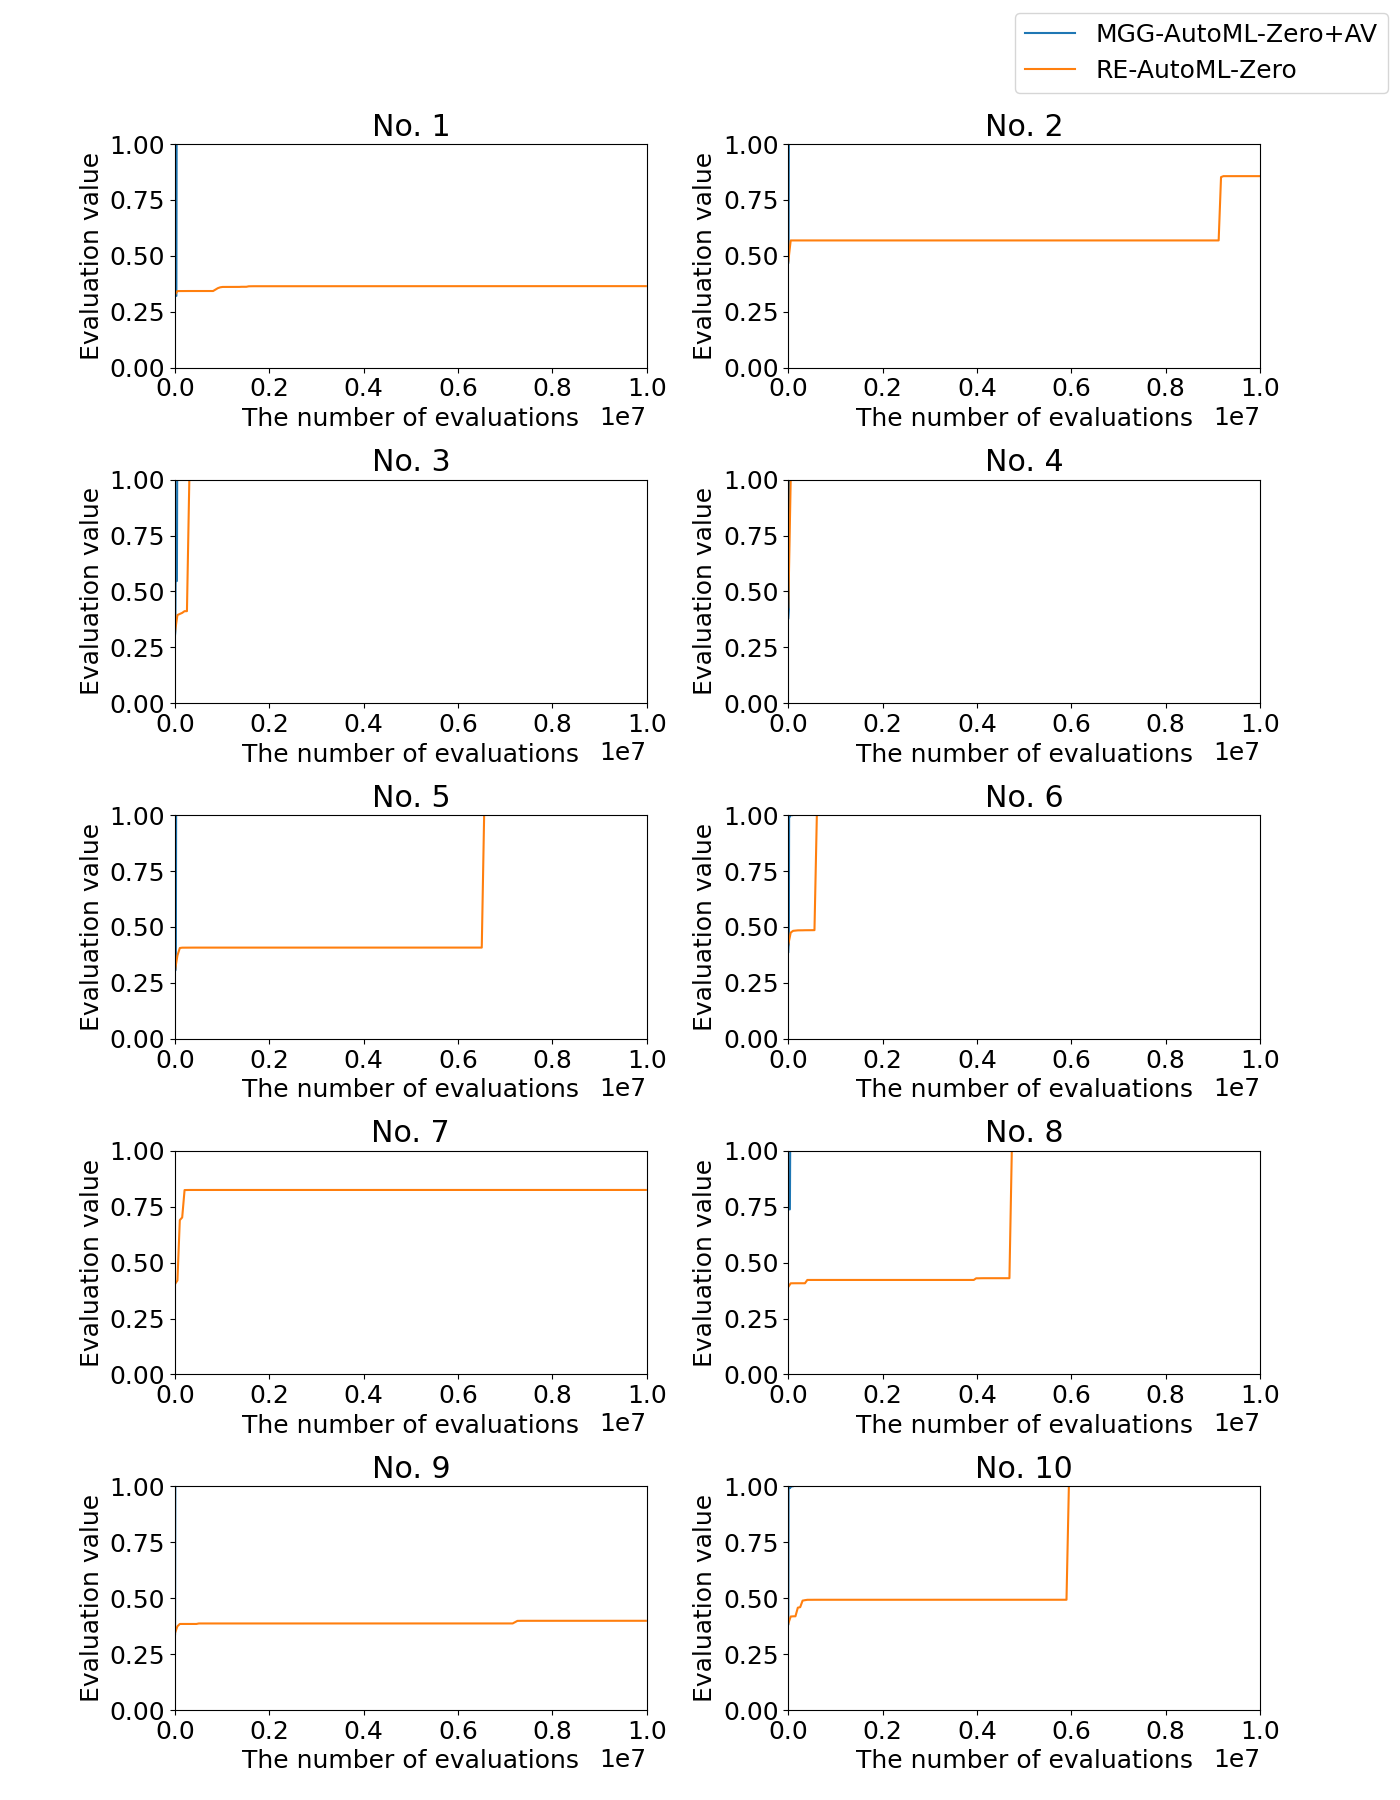
\includegraphics[width=14cm]{fitness_re_vs_mgg_av.png}
  \caption{第\ref{sec:mgg_automl_zero_av:exp}節の実験におけるMGG-AutoML-Zero+AVとAutoML-Zeroの集団内の最良個体の評価値の推移. 横軸は評価回数であり, 縦軸は集団内の最良個体の評価値である. }
  \label{fig:fitness_re_vs_mgg_av}
\end{figure}


\begin{figure}[tbp]
  \centering
  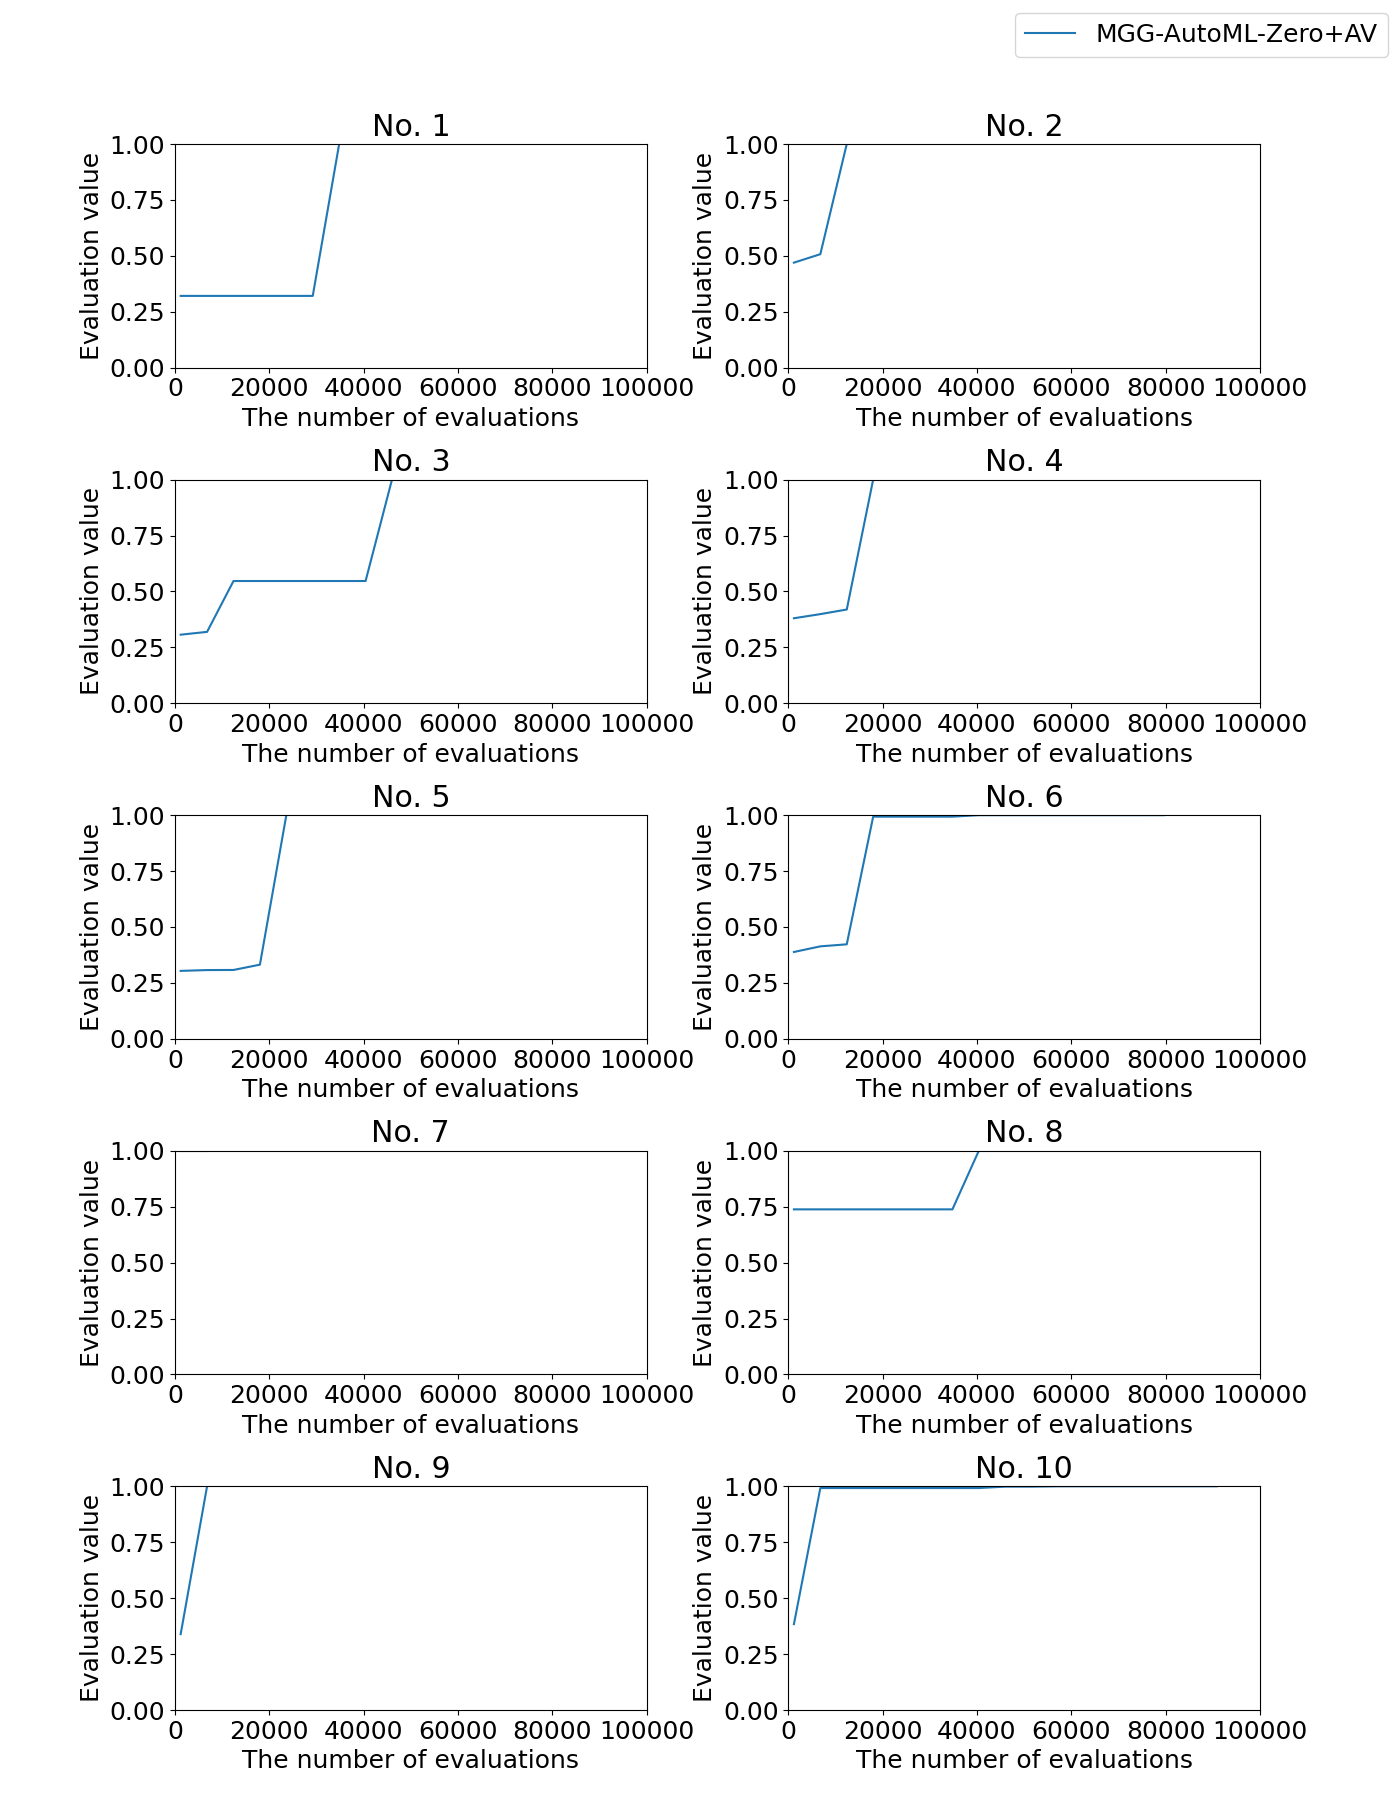
\includegraphics[width=14cm]{fitness_mgg_av.png}
  \caption{第\ref{sec:mgg_automl_zero_av:exp}節の実験におけるMGG-AutoML-Zero+AVの集団内の最良個体の評価値の推移. 横軸は評価回数であり, 縦軸は集団内の最良個体の評価値である. No. 7の試行は初期集団で評価値が0.999を超える個体が生成されているため, グラフが1.00の横軸と重なっていることに注意されたい. }
  \label{fig:fitness_mgg_av}
\end{figure}

第\ref{sec:mgg_automl_zero_av:exp}節で述べたように, MGG-AutoML-Zero+AVは, RE-AutoML-Zeroが半分の試行でしか成功しなかった線形回帰タスクの実験において, すべての試行を成功させ, 評価値も1/100未満にすることが出来た. この結果を詳細に分析するために, 第\ref{sec:mgg_automl_zero_av:exp}節の実験における集団内の最良個体の評価値の推移をFig.\ref{fig:fitness_re_vs_mgg_av}とFig.\ref{fig:fitness_mgg_av}を示す. 横軸は評価回数であり, 縦軸は集団内の最良個体の評価値である. Fig.\ref{fig:fitness_mgg_av}は, Fig.\ref{fig:fitness_re_vs_mgg_av}からMGG-AutoML-Zero+AVのみを取り出して拡大したグラフである. 集団内の最良個体の評価値の推移から読み取れるように, MGG-AutoML-Zero+AVは, どの試行でも評価回数が少ない段階で安定して評価値の改善が進んでいる. 一方, RE-AutoML-Zeroは特定の評価値付近で長期間改善されていない状況, すなわち局所解に陥っている状況が発生していることが分かる.


\subsection{MGGの有効性の確認と分析}\label{subsec:mgg_automl_zero_av:consideration:mgg}

本節では, 第\ref{sec:mgg_automl_zero_av:exp}節と同じ実験設定でMGG-AutoML-ZeroとRE-AutoML-Zeroの比較実験を行い, MGGの有効性を確認した上で, MGGよって集団の多様性がどの程度維持されるようになったのかを分析する. 以下, 第\ref{subsubsec:mgg_automl_zero_av:consideration:mgg:effect}節ではMGG-AutoML-ZeroとRE-AutoML-Zeroの比較実験によるMGGの有効性確認, 第\ref{subsubsec:mgg_automl_zero_av:consideration:mgg:analysis}節ではMGGによる多様性維持の分析を行う.

\subsubsection{MGGの有効性の確認}\label{subsubsec:mgg_automl_zero_av:consideration:mgg:effect}

本項では, 第\ref{sec:mgg_automl_zero_av:exp}節と同じ実験設定でMGG-AutoML-ZeroとRE-AutoML-Zeroの比較実験を行うことで, MGGの有効性を確認する. 本実験では, 初期集団の段階で多様性に差がでないよう初期集団をMGG-AutoML-ZeroとRE-AutoML-Zeroで揃えた. MGG-AutoML-ZeroとRE-AutoML-Zeroの比較実験結果を, Table.\ref{table:re_vs_mgg}に示す. Table.\ref{table:re_vs_mgg}の実験結果から, MGG-AutoML-ZeroはRE-AutoML-Zeroと比べて探索の成功率は40\%改善し, 評価回数は200,00回程度少なくなることが分かった. したがって, 本研究で提案したMGGによる世代交代は, アルゴリズムの探索に対して有効に作用することが確認された.

\begin{table}[tbp]
  \caption{第\ref{sec:mgg_automl_zero_av:exp}節と同じ実験設定でMGG-AutoML-ZeroとRE-AutoML-Zeroを比較した結果. }
  \label{table:re_vs_mgg}
  \centering
  \begin{tabular}{|c|cr|cr|}
    \hline
    \multirow{2}{*}{No. }
            & \multicolumn{2}{c|}{RE-AutoML-Zero} & \multicolumn{2}{c|}{MGG-AutoML-Zero}                  \\
            & 結果                                  & 評価回数                                 & 結果 & 評価回数      \\
    \hline \hline
    1       & 失敗                                  & -                                    & 成功 & 2,874,000 \\
    2       & 失敗                                  & -                                    & 成功 & 4,486,800 \\
    3       & 失敗                                  & -                                    & 成功 & 3,630,000 \\
    4       & 成功                                  & 51,600                               & 成功 & 1,412,400 \\
    5       & 成功                                  & 6,553,200                            & 成功 & 2,017,200 \\
    6       & 成功                                  & 606,000                              & 成功 & 7,006,800 \\
    7       & 失敗                                  & -                                    & 成功 & 2,571,600 \\
    8       & 成功                                  & 4,738,800                            & 成功 & 5,192,400 \\
    9       & 失敗                                  & -                                    & 失敗 & -         \\
    10      & 成功                                  & 5,948,400                            & 成功 & 908,400   \\
    \hline
    成功率     & \multicolumn{2}{c|}{$5/10$}         & \multicolumn{2}{c|}{$9/10$}                           \\
    \hline
    評価回数の平均 & \multicolumn{2}{c|}{3,579,600}      & \multicolumn{2}{c|}{3,344,400}                        \\
    \hline
  \end{tabular}
\end{table}

\subsubsection{MGGによる多様性維持の分析}\label{subsubsec:mgg_automl_zero_av:consideration:mgg:analysis}

本項では, 第\ref{subsubsec:mgg_automl_zero_av:consideration:mgg:effect}節で行った実験における集団内の最良個体の評価値の推移を確認することで, MGGの方が集団の多様性を維持できる世代交代モデルであることを確認する. RE-AutoML-ZeroおよびMGG-AutoML-Zeroそれぞれの集団内の最良個体の評価値の推移をFig.\ref{fig:fitness_re_vs_mgg}に示す. Fig.\ref{fig:fitness_re_vs_mgg}からMGG-AutoML-ZeroはRE-AutoML-Zeroに比べて, 段階的に集団内の最良個体の評価値が上昇していて, 局所解に陥りにくいことが分かる. これはMGG-AutoML-Zeroの方が, 集団の中に評価値を改善できる見込みがある形質を持った個体が, 集団内に多く含まれていることを意味する. つまり, MGG-AutoML-ZeroはRE-AutoML-Zeroに比べて, 集団の多様性を維持しやすいと考えられる.

\begin{figure}[tbp]
  \centering
  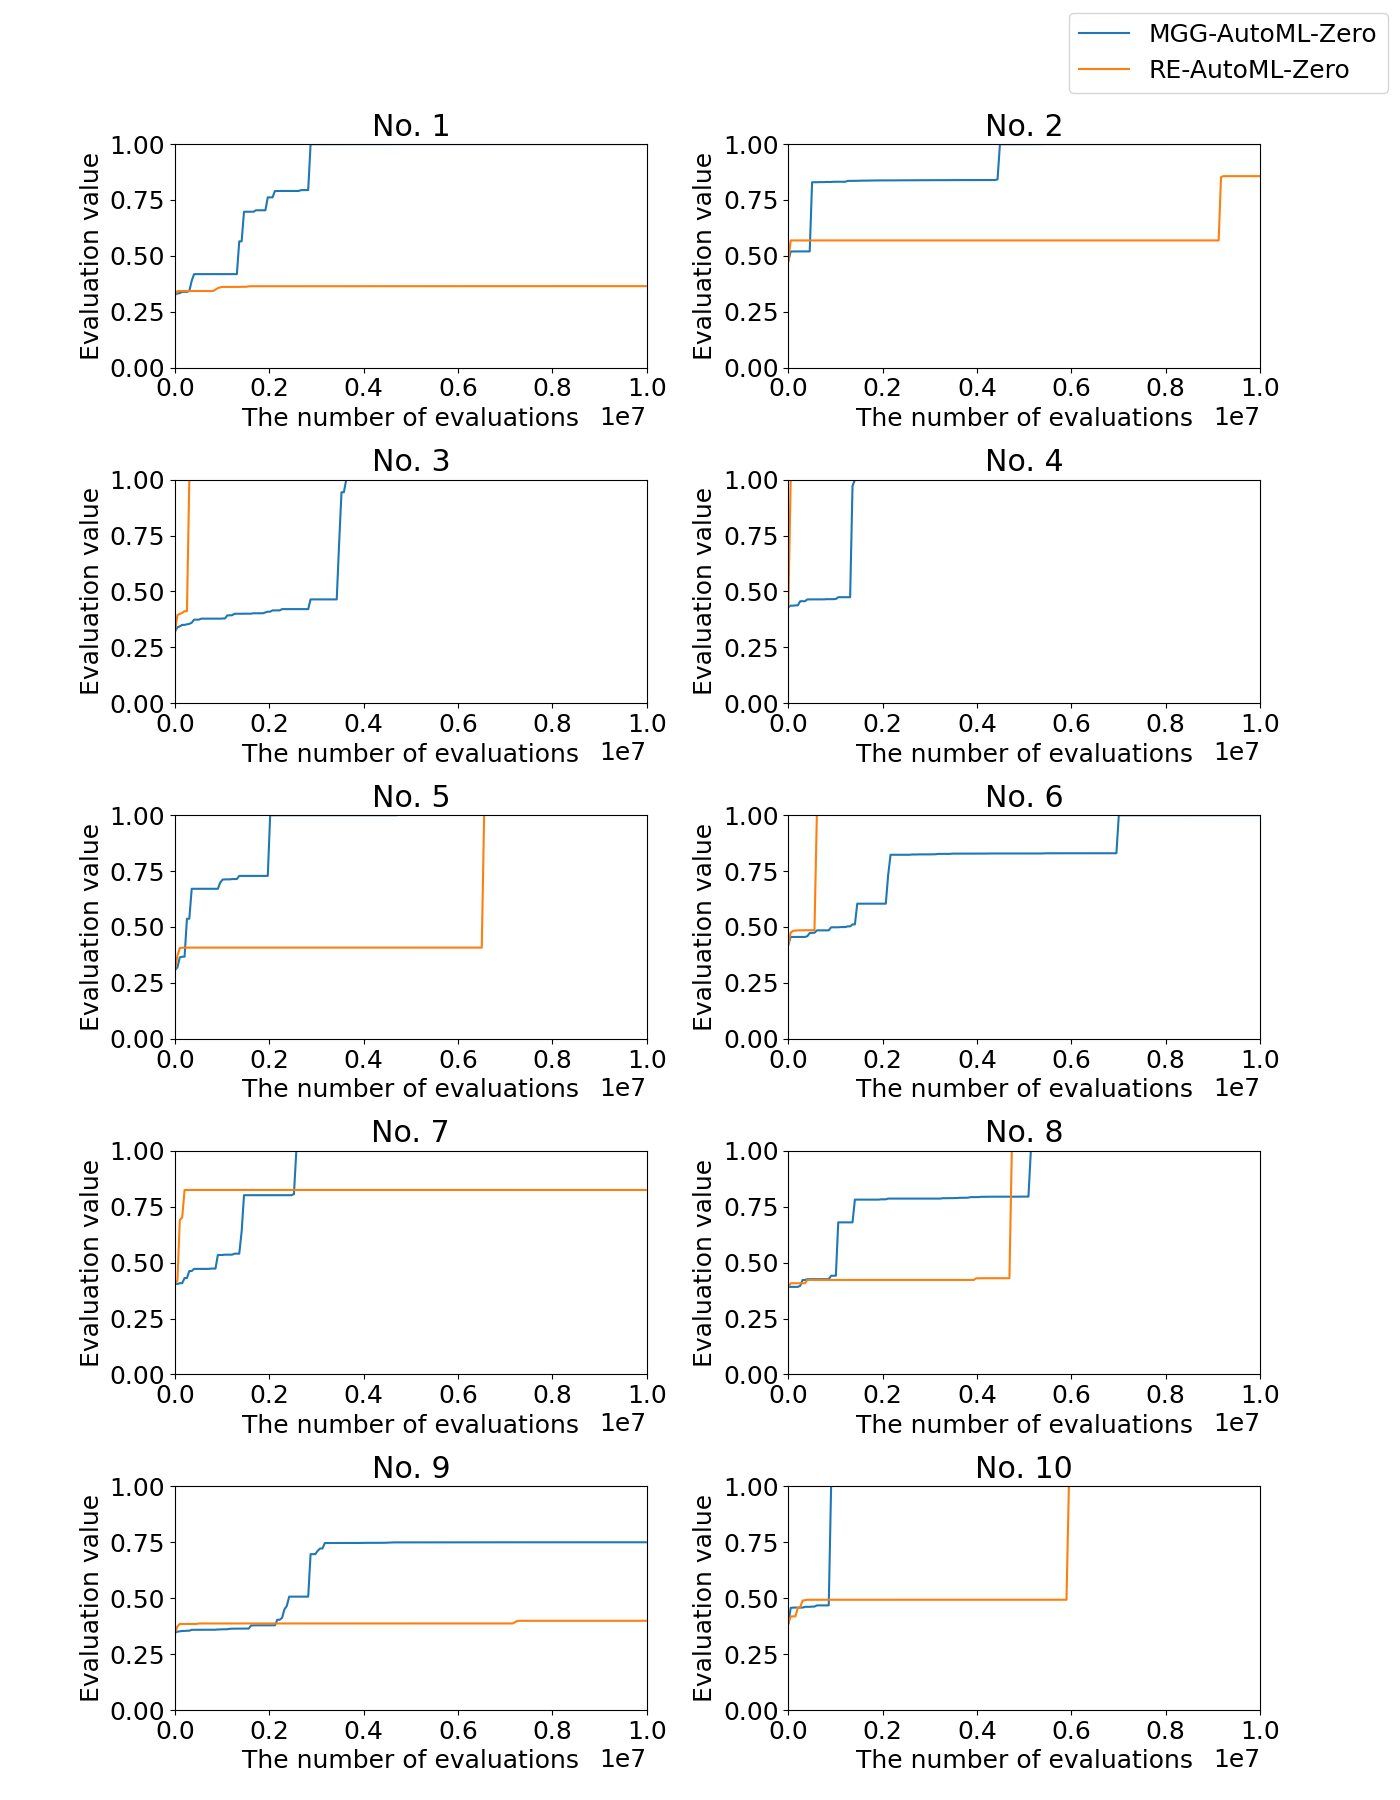
\includegraphics[width=14cm]{fitness_re_vs_mgg.png}
  \caption{第\ref{subsubsec:mgg_automl_zero_av:consideration:mgg:effect}節で行ったRE-AutoML-ZeroおよびMGG-AutoML-Zeroの比較実験における最良評価値の推移. 横軸は評価回数であり, 縦軸は集団内の最良個体の評価値である. }
  \label{fig:fitness_re_vs_mgg}
\end{figure}

\subsection{AVの有効性の確認と分析}\label{subsec:mgg_automl_zero_av:consideration:av}

本節では, 第\ref{sec:mgg_automl_zero_av:exp}節と同じ実験設定でMGG-AutoML-Zero+AVとMGG-AutoML-Zeroの比較実験を行い, AVの有効性を確認した上で, AVによってどの程度探索空間が削減されたのかを分析する. また, AVで行う各検証が有効であるかどうかを調べるために, MGG-AutoML-Zero+AVとMGG-AutoML-Zero+AVから一部の検証を外した手法を比較する. 以下, 第\ref{subsubsec:mgg_automl_zero_av:consideration:av:effect}節ではMGG-AutoML-Zero+AVとMGG-AutoML-Zeroの比較実験によるAVの有効性確認, 第\ref{subsubsec:mgg_automl_zero_av:consideration:av:analysis}節ではAVによる探索空間の削減に関する分析, 第\ref{subsubsec:mgg_automl_zero_av:consideration:av:each_analysis}節ではAVにおける各検証の有効性の確認を行う.

\subsubsection{AVの有効性の確認}\label{subsubsec:mgg_automl_zero_av:consideration:av:effect}

本項では, 第\ref{sec:mgg_automl_zero_av:exp}節と同じ実験設定でMGG-AutoML-Zero+AVとMGG-AutoML-Zeroの比較実験を行うことで, AVの有効性を確認する. MGG-AutoML-Zero+AVとMGG-AutoML-Zeroの比較実験結果を, Table.\ref{table:mgg_vs_mgg_av}に示す. Table.\ref{table:mgg_vs_mgg_av}の実験結果から, MGG-AutoML-Zero+AVはMGG-AutoML-Zeroが失敗していたNo. 9の試行に対しても成功し, 評価回数は$1/100$未満になることが分かった. したがって, 本研究で提案したアルゴリズムの検証AVは, アルゴリズムの探索に対して有効に作用することが確認された.

\begin{table}[tbp]
  \caption{RE-AutoML-Zero, MGG-AutoML-Zero, MGG-AutoML-Zero+AVで線形回帰アルゴリズムを探索した結果}
  \label{table:mgg_vs_mgg_av}
  \centering
  \begin{tabular}{|c|cr|cr|cr|}
    \hline
    \multirow{2}{*}{No. }
            & \multicolumn{2}{c|}{MGG-AutoML-Zero} & \multicolumn{2}{c|}{MGG-AutoML-Zero+AV}              \\
            & 結果                                   & 評価回数                                    & 結果 & 評価回数  \\
    \hline \hline
    1       & 成功                                   & 2,874,000                               & 成功 & 34800 \\
    2       & 成功                                   & 4,486,800                               & 成功 & 12400 \\
    3       & 成功                                   & 3,630,000                               & 成功 & 46000 \\
    4       & 成功                                   & 1,412,400                               & 成功 & 18000 \\
    5       & 成功                                   & 2,017,200                               & 成功 & 23600 \\
    6       & 成功                                   & 7,006,800                               & 成功 & 40400 \\
    7       & 成功                                   & 2,571,600                               & 成功 & 1200  \\
    8       & 成功                                   & 5,192,400                               & 成功 & 40400 \\
    9       & 失敗                                   & -                                       & 成功 & 6800  \\
    10      & 成功                                   & 908,400                                 & 成功 & 57200 \\
    \hline
    成功率     & \multicolumn{2}{c|}{$9/10$}          & \multicolumn{2}{c|}{$10/10$}                         \\
    \hline
    評価回数の平均 & \multicolumn{2}{c|}{3,344,400}       & \multicolumn{2}{c|}{28,080}                          \\
    \hline
  \end{tabular}
\end{table}

\subsubsection{AVの分析}\label{subsubsec:mgg_automl_zero_av:consideration:av:analysis}

本項では, AVによってどの程度探索空間を削減できたのかを定量化する. 第\ref{subsubsec:mgg_automl_zero_av:consideration:av:effect}節で行ったMGG-AutoML-Zero+AVの実験において, アルゴリズムの検証で妥当な機械学習アルゴリズムと判断された個体の割合を, 初期集団生成時と子個体生成時に分けて, Table.\ref{table:av_validation_rate}に示す. Table.\ref{table:av_validation_rate}から完全にランダムに個体を生成する初期集団生成時には, 0.0138\%アルゴリズムのみが実行可能解(妥当な機械学習アルゴリズム)であり, その他の99.9862\%は実行不可能解であった. このことから, アルゴリズムの検証を導入しない既存手法では, 探索空間の99.9862\%が冗長な探索空間になっていたことが分かる. また, 妥当な機械学習アルゴリズムの突然変異によって個体を生成する子個体生成では, 妥当な機械学習アルゴリズム生成される割合は0.0264\%であった. すなわち, RE-AutoML-Zeroの突然変異オペレータは, 実行可能解を不可能解にしてしまう確率が99.97\%を超える破壊的なオペレータであることが分かった.

\begin{table}[tbp]
  \caption{第\ref{subsubsec:mgg_automl_zero_av:consideration:av:effect}節で行ったMGG-AutoML-Zero+AVの実験において, アルゴリズムの検証で実行可能解(妥当な機械学習アルゴリズム)と判断された個体の割合. 初期集団生成時と子個体生成時に分けて示している. }
  \label{table:av_validation_rate}
  \centering
  \begin{tabular}{|c|r|r|}
    \hline
    No & 初期集団生成時  & 子個体生成時   \\
    \hline \hline
    1  & 0.0140\% & 0.0260\% \\
    2  & 0.0137\% & 0.0269\% \\
    3  & 0.0133\% & 0.0262\% \\
    4  & 0.0142\% & 0.0261\% \\
    5  & 0.0138\% & 0.0258\% \\
    6  & 0.0143\% & 0.0261\% \\
    7  & 0.0131\% & 0.0276\% \\
    8  & 0.0139\% & 0.0266\% \\
    9  & 0.0138\% & 0.0263\% \\
    10 & 0.0137\% & 0.0262\% \\
    \hline
    平均 & 0.0138\% & 0.0264\% \\
    \hline
  \end{tabular}
\end{table}

\subsubsection{AVで行う各検証の有効性の確認}\label{subsubsec:mgg_automl_zero_av:consideration:av:each_analysis}

本節では, AVの各検証の有効性を確認するために, AVから特定の検証Xを除外したアルゴリズム検証$\mathrm{AV}-X$を用いて第\ref{sec:mgg_automl_zero_av:exp}節と同じ実験を行う. つまり, 探索に用いる手法は, MGG-AutoML-Zero+($\mathrm{AV}-X$)となる. $X$には, PFV, $\mathrm{PLV}_{v0}$, $\mathrm{LPV}_{s0}$等の検証名を代入する. 検証名と検証内容の対応関係の詳細は第\ref{subsubsec:mgg_automl_zero_av:suggest:av:basic}節を参照されたい.

Table.\ref{table:av-x}にアルゴリズムの検証法ごとに, 10試行分の実験を行った結果を示す. 探索の成功率は10試行の中で成功した探索の割合, 平均の評価回数は成功試行の探索が要した評価回数の平均, 平均の実行可能解の割合は, 初期集団生成時と子個体生成時それぞれで実行可能解が生成された割合の平均を意味する. Table.\ref{table:av-x}より, AVを検証法として導入したときが最も平均の評価回数が小さいことが分かる. ただし, 今回の実験においてはPredict関数の命令数が1で固定されているため, $\mathrm{PFV}$は$\mathrm{PLV}_{v0}$や$\mathrm{PLV}_{LP}$の検証に包含されてしまうため, $\mathrm{AV}-\mathrm{PFV}$とAVが同じ結果になった. しかし, $\mathrm{PFV}$はPredictに含まれる関数が複数になった場合, 他の検証をするために必要な検証であるため, 欠かすことは出来ない. 以上のことから, AVに含まれるすべての検証が探索に対して有効であったことが従う.

\begin{table}[tbp]
  \caption{検証法ごとに第\ref{sec:mgg_automl_zero_av:exp}節の実験を行った結果. 探索の成功率は10試行の中で成功した探索の割合, 平均の評価回数は成功試行の探索が要した評価回数の平均, 平均の実行可能解の割合は, 初期集団生成時と子個体生成時それぞれで実行可能解が生成された割合の平均を意味する. }
  \label{table:av-x}
  \centering
  \begin{tabular}{|l|cr|rr|}
    \hline
    \multirow{2}{*}{検証手法}                    & \multirow{2}{*}{探索の成功率}            & \multirow{2}{*}{平均の評価回数}
                                             & \multicolumn{2}{c|}{平均の実行可能解の生成割合}                                                      \\
                                             &                                    &                          & 初期集団生成時    & 子個体生成時     \\
    \hline \hline
    なし                                       & $9/10$                             & 3,344,400                & 100.0000\% & 100.0000\% \\
    $\mathrm{AV}$                            & $10/10$                            & 28,080                   & 0.0138\%   & 0.0264\%   \\
    \hline
    $\mathrm{AV}-\mathrm{PFV}$               & $10/10$                            & 28,080                   & 0.0138\%   & 0.0264\%   \\
    $\mathrm{AV}-\mathrm{PLV}_{v0}$          & $10/10$                            & 62,800                   & 0.1055\%   & 0.2174\%   \\
    $\mathrm{AV}-\mathrm{PLV}_\mathrm{LP}$   & $6/10$                             & 2,580,000                & 55.6808\%  & 80.6304\%  \\
    $\mathrm{AV}-\mathrm{LPV}_\mathrm{prev}$ & $10/10$                            & 138400                   & 0.4088\%   & 0.8165\%   \\
    $\mathrm{AV}-\mathrm{LPV}_{s0}$          & $10/10$                            & 162480                   & 0.3710\%   & 0.7364\%   \\
    $\mathrm{AV}-\mathrm{LPV}_{s1}$          & $10/10$                            & 197760                   & 0.4205\%   & 0.8504\%   \\
    $\mathrm{AV}-\mathrm{LPV}_{v0}$          & $10/10$                            & 151840                   & 0.3030\%   & 0.6081\%   \\
    \hline
  \end{tabular}
\end{table}

\section{おわりに}
本章では, Estebanらが提案した手法であるRE-AutoML-Zeroの問題点を述べ, それらの問題を解決する手法MGG-AutoML-Zero+AVを提案した. そして, MGG-AutoML-Zero+AVとRE-AutoML-Zeroの比較実験および考察を通じて, 提案手法の有効性を確認した. 以下では, 本章の内容を簡単に取りまとめる.

\subsection{既存手法の問題点}\label{subsec:mgg_auto_ml_zero:end:problem}

本章では, 第\ref{chap:problem}章でAutoML-Zeroの問題設定を説明した上で, Estebanらが提案した手法であるRE-AutoML-Zeroに関する問題点を2つ指摘した. 1つめは, RE-AutoML-Zeroで用いられている世代交代モデルREは多様性を失いやすい点である. REは, 複製選択で選択圧が強く掛かったり, 生存選択で無条件で淘汰する個体が淘汰され, 淘汰される個体とは関係ない個体が生存したりすることがあり, それが集団の多様性の低下に繋がっている可能性を指摘した. 2つめとしては, 妥当ではない機械学習アルゴリズムが探索対象となっており, 探索空間が冗長になっている問題点を指摘した. RE-AutoML-Zeroでは, 学習対象のパラメータや入力ベクトルが予測のラベルを求めるのに使われていなくても, 探索対象として扱い評価を行っていた. しかし, このような妥当ではないアルゴリズムは, いかなる機械学習のタスクについても, 除外されるべきであるため, 探索対象に含める必要がないことを論じた.

\subsection{既存手法の問題点に対処した手法の提案}\label{subsec:mgg_auto_ml_zero:end:suggest}

本章の第\ref{sec:mgg_automl_zero_av:suggest}節では, 既存手法の問題点に対処した手法を提案した. はじめに, 集団の多様性が失われやすい世代交代であるREを, 佐藤らが提案したMGGに置き換えることを提案した. MGGは複製選択時の選択圧を無くした上で, 生存選択時には次の世代に追加される個体として, 淘汰された個体自身または家族が選択される世代交代モデルであり, 既存手法の世代交代モデルに関する問題に対処できる手法である. また, 妥当ではない機械学習アルゴリズムが探索対象となる問題については, 妥当なアルゴリズムであることを検証して, 妥当ではないアルゴリズムを実行不可能解として扱う手法を提案した.

\subsection{提案手法の性能評価と考察}\label{subsec:mgg_auto_ml_zero:end:result}

本章では, 第\ref{sec:mgg_automl_zero_av:exp}節で提案手法が既存手法よりも線型回帰タスクの問題において優れていることを確認した上で, 第\ref{sec:mgg_automl_zero_av:consideration}節で既存手法の問題点に対して対処できていることを分析によって明らかにした. 第\ref{sec:mgg_automl_zero_av:exp}節の実験結果では, 既存手法が50\%しか成功しない線型回帰タスクに対して, 提案手法は100\%成功した上で評価回数も既存手法の1/100未満になることを確認した.

第\ref{subsec:mgg_automl_zero_av:consideration:mgg}項では, 世代交代モデルとしてMGGを導入したMGG-AutoML-Zeroと既存手法のRE-AutoML-Zeroの2つを比較をすることでMGGの有効性を確認した. MGG-AutoML-ZeroはRE-AutoML-Zeroに比べて成功率が40\%高く, 探索に必要な評価回数も200,000回以上少ないことが分かった. また, 集団内の最良個体の評価値の推移を比較することで, 集団の多様性がREに比べてMGGの方が維持できていることを確認した.

第\ref{subsec:mgg_automl_zero_av:consideration:av}項では, アルゴリズムの検証に関する有効性をMGG-AutoML-ZeroとMGG-AutoML-Zero+AVを比較することで確認した. MGG-AutoML-Zero+AVは, MGG-AutoML-Zeroで解けなかった試行が解けるようになり, 評価回数も1/100未満になることが分かった. 加えて, アルゴリズムの検証で実行不可能解となるアルゴリズムの割合を調べることで, 探索空間をどの程度削減できているのかを分析した. 分析の結果, 既存手法の探索空間の99.98\%以上が削減できていることが分かった.

\appendix

\chapter{命令セット}

本研究のアルゴリズムを構成するための命令セットをTable.\ref{table:instructions}に示す. この命令セットはEstebanらの論文\cite{automl_zero}に使われている命令セットと同様である.

\begin{center}
  {\renewcommand\arraystretch{1.9}
    {\scriptsize
      \begin{longtable}{l|l|lc|lc|l}
        \caption{アルゴリズムの各関数Setup, Predict, Learnを構成する命令の一覧. Estebanらの論文\cite{automl_zero}に示されている命令セットと同様である. }
        \\
        \hline
        \multirow{2}{*}{ID}
             & \multirow{2}{*}{コード例}
             & \multicolumn{2}{c|}{入力}                    & \multicolumn{2}{c|}{出力}
             & \multirow{2}{*}{説明}                                                                                                                                                                          \\
             &                                            & 変数/型                    & 定数              & 変数/型       & 添字                                                                                     \\
        \hline \hline
        \endfirsthead
        \hline
        \multirow{2}{*}{命令ID}
             & \multirow{2}{*}{コード例}
             & \multicolumn{2}{c|}{入力}                    & \multicolumn{2}{c|}{出力}
             & \multirow{2}{*}{説明}                                                                                                                                                                          \\
             &                                            & 変数/型                    & 定数              & 変数/型       & 添字                                                                                     \\
        \hline \hline
        \endhead

        \label{table:instructions}
        OP0  & no\_op                                     & -                       & -               & -          & -     & -                                                                              \\
        OP1  & $s2 = s3 + s0$                             & $a,b$/scalars           & -               & $c$/scalar & -     & $s_c = s_a + s_b$                                                              \\
        OP2  & $s4 = s0 - s1$                             & $a,b$/scalars           & -               & $c$/scalar & -     & $s_c = s_a - s_b$                                                              \\
        OP3  & $s8 = s5 * s5$                             & $a,b$/scalars           & -               & $c$/scalar & -     & $s_c = s_a s_b$                                                                \\
        OP4  & $s7 = s5 / s2$                             & $a,b$/scalars           & -               & $c$/scalar & -     & $s_c = s_a / s_b$                                                              \\
        OP5  & $s8 = \mathrm{abs}(s0)$                    & $a$/scalar              & -               & $b$/scalar & -     & $s_b = |s_a|$                                                                  \\
        OP6  & $s4 = 1/ s8$                               & $a$/scalar              & -               & $b$/scalar & -     & $s_b = 1/s_a$                                                                  \\
        OP7  & $s5 = \mathrm{sin}(s4)$                    & $a$/scalar              & -               & $b$/scalar & -     & $s_b = \mathrm{sin}(s_a)$                                                      \\
        OP8  & $s1 = \mathrm{cos}(s4)$                    & $a$/scalar              & -               & $b$/scalar & -     & $s_b = \mathrm{cos}(s_a)$                                                      \\
        OP9  & $s0 = \mathrm{tan}(s4)$                    & $a$/scalar              & -               & $b$/scalar & -     & $s_b = \mathrm{tan}(s_a)$                                                      \\
        OP10 & $s0 = \mathrm{arcsin}(s4)$                 & $a$/scalar              & -               & $b$/scalar & -     & $s_b = \mathrm{arcsin}(s_a)$                                                   \\
        OP11 & $s2 = \mathrm{arccos}(s0)$                 & $a$/scalar              & -               & $b$/scalar & -     & $s_b = \mathrm{arccos}(s_a)$                                                   \\
        OP12 & $s4 = \mathrm{arctan}(s0)$                 & $a$/scalar              & -               & $b$/scalar & -     & $s_b = \mathrm{arctan}(s_a)$                                                   \\
        OP13 & $s1 = \mathrm{exp}(s2)$                    & $a$/scalar              & -               & $b$/scalar & -     & $s_b = e^{s_a}$                                                                \\
        OP14 & $s0 = \mathrm{log}(s3)$                    & $a$/scalar              & -               & $b$/scalar & -     & $s_b = \log s_a$                                                               \\
        OP15 & $s3 = \mathrm{heaviside}(s0)$              & $a$/scalar              & -               & $b$/scalar & -     & $s_b = \mathbbm{1}_{\mathbb{R}+}(s_a)$                                         \\
        OP16 & $v2 = \mathrm{heaviside}(v2)$              & $a$/vector              & -               & $b$/vector & -     & $\forall i,\bm{v}_b^{(i)} = \mathbbm{1}_{\mathbb{R}+}(\bm{v}_a^{(i)})$         \\
        OP17 & $m7 = \mathrm{heaviside}(m3)$              & $a$/matrix              & -               & $b$/matrix & -     & $\forall i, jM_b^{(i, j)} = \mathbbm{1}_{\mathbb{R}+}(M_a^{(i, j)})$           \\
        OP18 & $v1 = s7 * v1$                             & $a,b$/sc, vec           & -               & $c$/vector & -     & $\bm{v}_c = s_a \bm{v}_b$                                                      \\
        OP19 & $v1 = \mathrm{bcast}(s3)$                  & $a$/scalar              & -               & $b$/vector & -     & $ \forall i,\bm{v}_b^{(i)} = s_a $                                             \\
        OP20 & $v5 = 1/v7$                                & $a$/vector              & -               & $b$/vector & -     & $ \forall i,\bm{v}_b^{(i)} = 1/s_a^{(i)} $                                     \\
        OP21 & $s0 = \mathrm{norm}(v3)$                   & $a$/scalar              & -               & $b$/vector & -     & $s_b = \left\| \bm{v}_a \right\|$                                              \\
        OP22 & $v3 = \mathrm{abs}(v3)$                    & $a$/vector              & -               & $b$/vector & -     & $\forall i,\bm{v}_b^{(i)} = \left| \bm{v}_a^{(i)} \right|$                     \\

        OP23 & $v5 = v0 + v9$                             & $a,b$/vectors           & -               & $c$/scalar & -     & $\bm{v}_c = \bm{v}_a + \bm{v}_b$                                               \\
        OP24 & $v1 = v0 - v9$                             & $a,b$/vectors           & -               & $c$/scalar & -     & $\bm{v}_c = \bm{v}_a - \bm{v}_b$                                               \\
        OP25 & $v8 = v0 * v9$                             & $a,b$/vectors           & -               & $c$/scalar & -     & $\forall i,\bm{v}_c^{(i)} = \bm{v}_a^{(i)} \bm{v}_b^{(i)}$                     \\
        OP26 & $v9 = v8 / v2$                             & $a,b$/vectors           & -               & $c$/scalar & -     & $\forall i,\bm{v}_c^{(i)} = \bm{v}_a^{(i)} / \bm{v}_b^{(i)}$                   \\
        OP27 & $s6 = \mathrm{dot}(v1, v5)$                & $a,b$/vectors           & -               & $c$/scalar & -     & $s_c = \bm{v}_a^T \bm{v}_b$                                                    \\
        OP28 & $m1 = \mathrm{outer}(v6, v5)$              & $a,b$/vectors           & -               & $c$/matrix & -     & $M_c = \bm{v}_a\bm{v}_b^T$                                                     \\
        OP29 & $m1 = a4 * m2$                             & $a,b$/sc/mat            & -               & $c$/matrix & -     & $M_c = s_a M_b$                                                                \\
        OP30 & $m3 = 1/m0$                                & $a$/matrix              & -               & $b$/matrix & -     & $ \forall i,j, M_b^{(i,j)} = 1/M_a^{(i, j)} $                                  \\
        OP31 & $v6 = \mathrm{dot}(m1, v0)$                & $a,b$/mat/vec           & -               & $c$/vector & -     & $\bm{v}_c = M_a \bm{v}_b$                                                      \\
        OP32 & $m2 = \mathrm{bcast}(v0, \mathrm{axis}=0)$ & $a$/vector              & -               & $b$/matrix & -     & $\forall i,j,M_b^{(i,j)}= \bm{v}_a^{(i)}$                                      \\
        OP33 & $m2 = \mathrm{bcast}(v0, \mathrm{axis}=1)$ & $a$/vector              & -               & $b$/matrix & -     & $\forall i,j,M_b^{(j,i)}= \bm{v}_a^{(i)}$                                      \\
        OP34 & $s2 = \mathrm{norm}(m1)$                   & $a$/matrix              & -               & $b$/scalar & -     & $s_b = \left\| \bm{v}_a \right\|$                                              \\
        OP35 & $v4 = \mathrm{norm}(m7, \mathrm{axis}=0)$  & $a$/matrix              & -               & $b$/vector & -     & $\forall i, \bm{v}_b^{(i)} = \left\| M_a^{(i, \cdot)} \right\|$                \\
        OP36 & $v4 = \mathrm{norm}(m7, \mathrm{axis}=1)$  & $a$/matrix              & -               & $b$/vector & -     & $\forall i, \bm{v}_b^{(i)} = \left\| M_a^{(\cdot, i)} \right\|$                \\
        OP37 & $m9 = \mathrm{transpose}(m3)$              & $a$/matrix              & -               & $b$/matrix & -     & $M_b = M_a^T$                                                                  \\
        OP38 & $m1 = \mathrm{abs}(m8)$                    & $a$/matrix              & -               & $b$/matrix & -     & $ \forall i,j, M_b^{(i,j)} = \left|M_a^{(i, j)}\right| $                       \\
        OP39 & $m2 = m2 + m0$                             & $a,b$/matrixes          & -               & $c$/matrix & -     & $M_c = M_a + M_b$                                                              \\
        OP40 & $m2 = m3 - m1$                             & $a,b$/matrixes          & -               & $c$/matrix & -     & $M_c = M_a - M_b$                                                              \\
        OP41 & $m3 = m2 * m3$                             & $a,b$/matrixes          & -               & $c$/matrix & -     & $\forall i,j, M_c^{(i,j)} = M_a^{(i,j)} M_b^{(i,j)}$                           \\
        OP42 & $m4 = m2 / m4$                             & $a,b$/matrixes          & -               & $c$/matrix & -     & $\forall i,j, M_c^{(i,j)} = M_a^{(i,j)} / M_b^{(i,j)}$                         \\
        OP43 & $m5 = \mathrm{matmul}(m5, m7)$             & $a,b$/matrixes          & -               & $c$/matrix & -     & $M_c = M_a M_b$                                                                \\
        OP44 & $s1 = \mathrm{minimun}(s2, s3)$            & $a,b$/scalars           & -               & $c$/scalar & -     & $s_c = \min{(s_a,s_b)}$                                                        \\
        OP45 & $v4 = \mathrm{minimun}(v3, v9)$            & $a,b$/vectors           & -               & $c$/vector & -     & $\forall i,\bm{v}_c^{(i)} = \min{\left(\bm{v}_a^{(i)},\bm{v}_b^{(i)}\right)}$  \\
        OP46 & $m5 = \mathrm{minimun}(m5, m7)$            & $a,b$/matrixes          & -               & $c$/matrix & -     & $\forall i,j,M_c^{(i,j)} = \min{\left(M_a^{(i,j)}, M_b^{(i,j)}\right)}$        \\
        OP47 & $s8 = \mathrm{maximum}(s3, s0)$            & $a,b$/scalars           & -               & $c$/scalar & -     & $s_c = \max{(s_a,s_b)}$                                                        \\
        OP48 & $v7 = \mathrm{maximum}(v3, v6)$            & $a,b$/vectors           & -               & $c$/vector & -     & $\forall i, \bm{v}_c^{(i)} = \max{\left(\bm{v}_a^{(i)},\bm{v}_b^{(i)}\right)}$ \\
        OP49 & $m7 = \mathrm{maximum}(m1, m0)$            & $a,b$/matrixes          & -               & $c$/matrix & -     & $\forall i,j, M_c^{(i,j)} = \max{\left(M_a^{(i,j)}, M_b^{(i,j)}\right)}$       \\
        OP50 & $s2 = \mathrm{mean}(v2)$                   & $a$/vector              & -               & $b$/scalar & -     & $s_b = \mathrm{mean}\left(\bm{v}_a\right)$                                     \\
        OP51 & $s2 = \mathrm{mean}(m8)$                   & $a$/matrix              & -               & $b$/scalar & -     & $s_b = \mathrm{mean}\left(M_a\right)$                                          \\
        OP52 & $v1 = \mathrm{mean}(m2, \mathrm{axis}=0)$  & $a$/matrix              & -               & $b$/vector & -     & $\forall i,\bm{v}_b^{(i)} = \mathrm{mean}\left(M_a^{(i,\cdot)}\right)$         \\
        OP53 & $v3 = \mathrm{stdev}(m2, \mathrm{axis}=0)$ & $a$/matrix              & -               & $b$/vector & -     & $\forall i,\bm{v}_b^{(i)} = \mathrm{stdev}\left(M_a^{(i,\cdot)}\right)$        \\
        OP54 & $s3 = \mathrm{stdev}(v3)$                  & $a$/vector              & -               & $b$/scalar & -     & $s_b = \mathrm{stdev}\left(\bm{v}_a\right)$                                    \\
        OP55 & $s4 = \mathrm{stdev}(m0)$                  & $a$/matrix              & -               & $b$/scalar & -     & $s_b = \mathrm{stdev}\left(M_a\right)$                                         \\
        OP56 & s2 = 0.7                                   & -                       & $ \gamma $      & $a$/scalar & -     & $s_a = \gamma $                                                                \\
        OP57 & v3[5] = -2.4                               & -                       & $\gamma$        & $a$/vector & $i$   & $\bm{v}_a^{(i)} = \gamma $                                                     \\
        OP58 & m2[5,1] = -0.03                            & -                       & $\gamma$        & $a$/matrix & $i,j$ & $M^{(i,j)}= \gamma$                                                            \\
        OP59 & $s4 = \mathrm{uniform}(-1,1)$              & -                       & $\alpha, \beta$ & $a$/scalar & -     & $s_a = \mathcal{U}(\alpha, \beta)$                                             \\
        OP60 & $v1 = \mathrm{uniform}(0.4,0.8)$           & -                       & $\alpha, \beta$ & $a$/vector & -     & $\forall i, \bm{v}_a^{(i)} = \mathcal{U}(\alpha, \beta)$                       \\
        OP61 & $m0 = \mathrm{uniform}(-0.5,0.6)$          & -                       & $\alpha, \beta$ & $a$/vector & -     & $\forall i, j, M_a^{(i, j)} = \mathcal{U}(\alpha, \beta)$                      \\
        OP62 & $s4 = \mathrm{gaussian}(0.1,0.7)$          & -                       & $\mu, \sigma$   & $a$/scalar & -     & $s_a = \mathcal{N}(\mu, \sigma)$                                               \\
        OP63 & $v8 = \mathrm{gaussian}(0.4,1)$            & -                       & $\mu, \sigma$   & $a$/vector & -     & $\forall i, \bm{v}_a^{(i)} = \mathcal{N}(\mu, \sigma)$                         \\
        OP64 & $m2 = \mathrm{gaussian}(-2,1.3)$           & -                       & $\mu, \sigma$   & $a$/vector & -     & $\forall i, j, M_a^{(i, j)} = \mathcal{N}(\mu, \sigma)$                        \\
        \hline
      \end{longtable}}}

\end{center}

\bibliographystyle{jplain}
\bibliography{ref}


\end{document}

